\section{Numerical simulation}

Below we have a simulation of the Allen--Cahn equation by Paul Kühnert in 
\cite{kuehner_simulation} through a finite elements method using the FEniCS 
environment. 
All simulations were run on a uniform unit square mesh of 
size $ 100 \times 100 $. The equation (\ref{ac_weak_equation}) is solved 
using a central difference time stepping scheme with time step size $ dt = 5 
\times 10^{ - 5 } $ and a Newton solver to handle the nonlinearity.
The potential used is $ W ( u ) = ( u^2 - 1 )^2 $. As initial data piecewise 
linear approximations with an $ \varepsilon $-slope of the indicator function 
of a ball have been chosen for \Cref{numerical_simulation_bump}. In 
\Cref{numerical_simulation_dumbbell} the initial data is similar but instead 
with a union of two balls.
\begin{figure}[h]
	\centering
	
	\begin{subfigure}[b]{0.3\linewidth}
		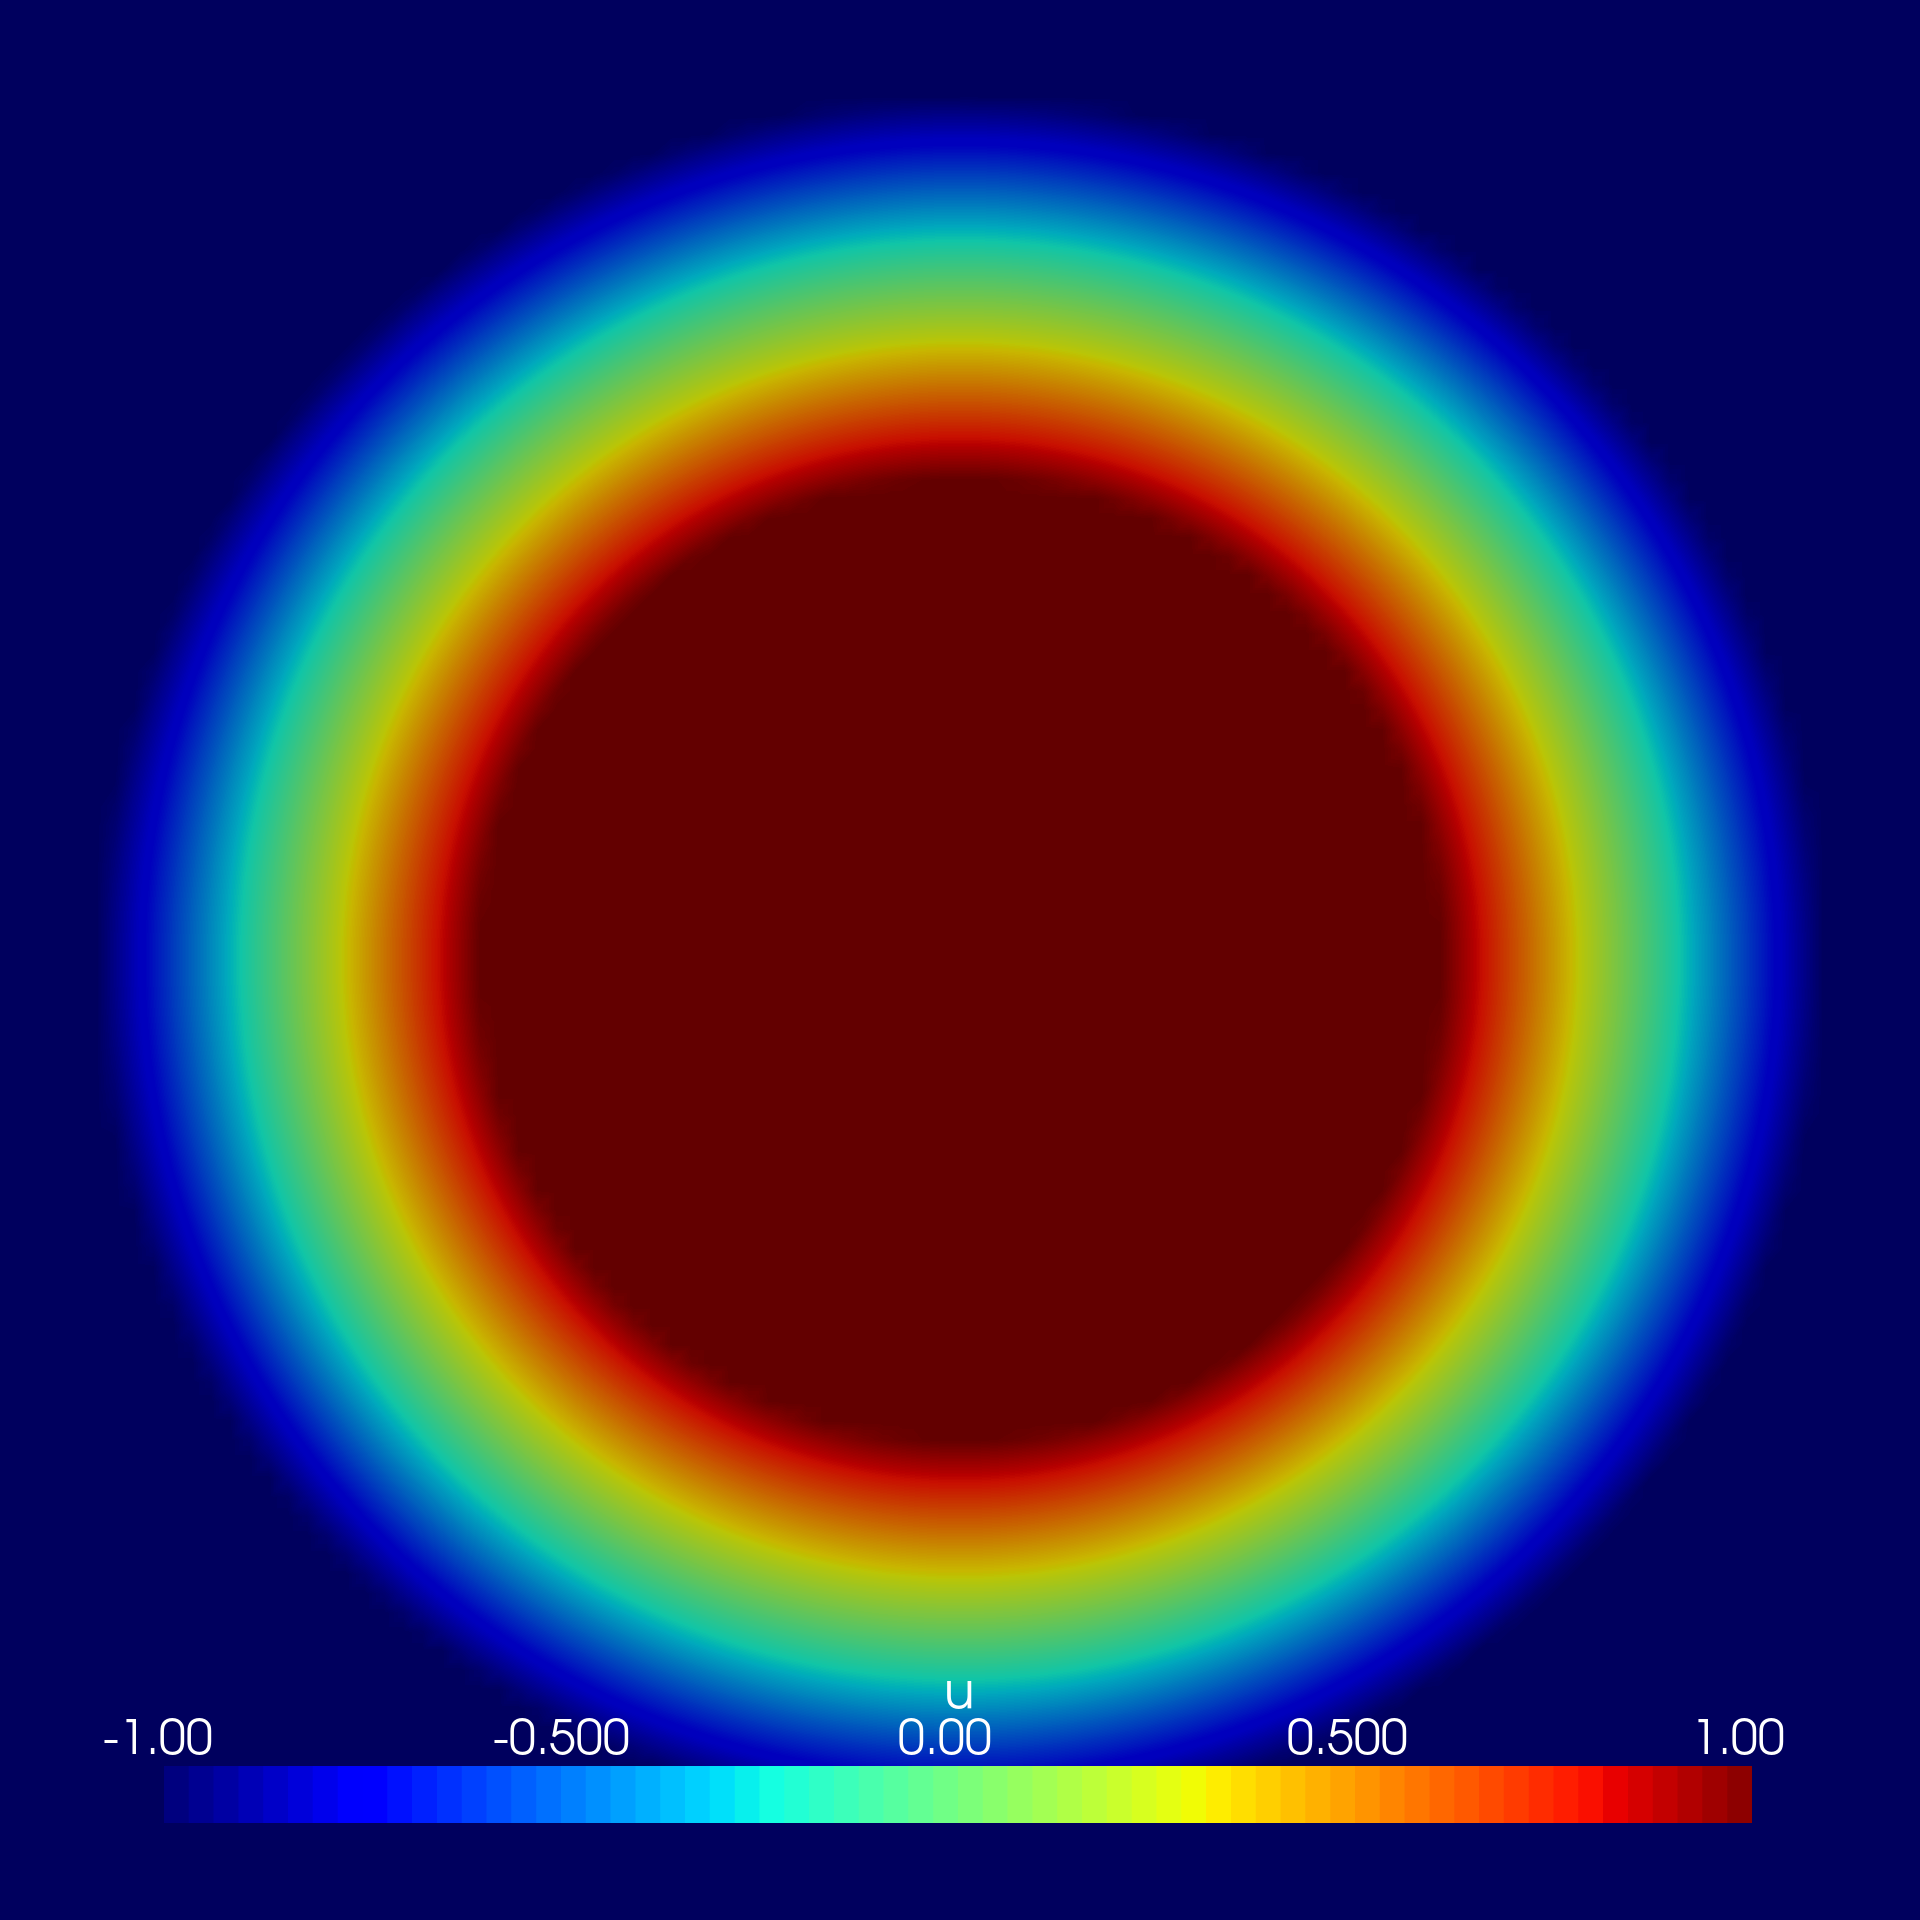
\includegraphics[width=\linewidth]{numerical_simulation/bump/eps_0.2000000.vtu}
		\caption{$ \varepsilon = 0.2, t = 0 $}
	\end{subfigure}
	\hfill
	\begin{subfigure}[b]{0.3\linewidth}
		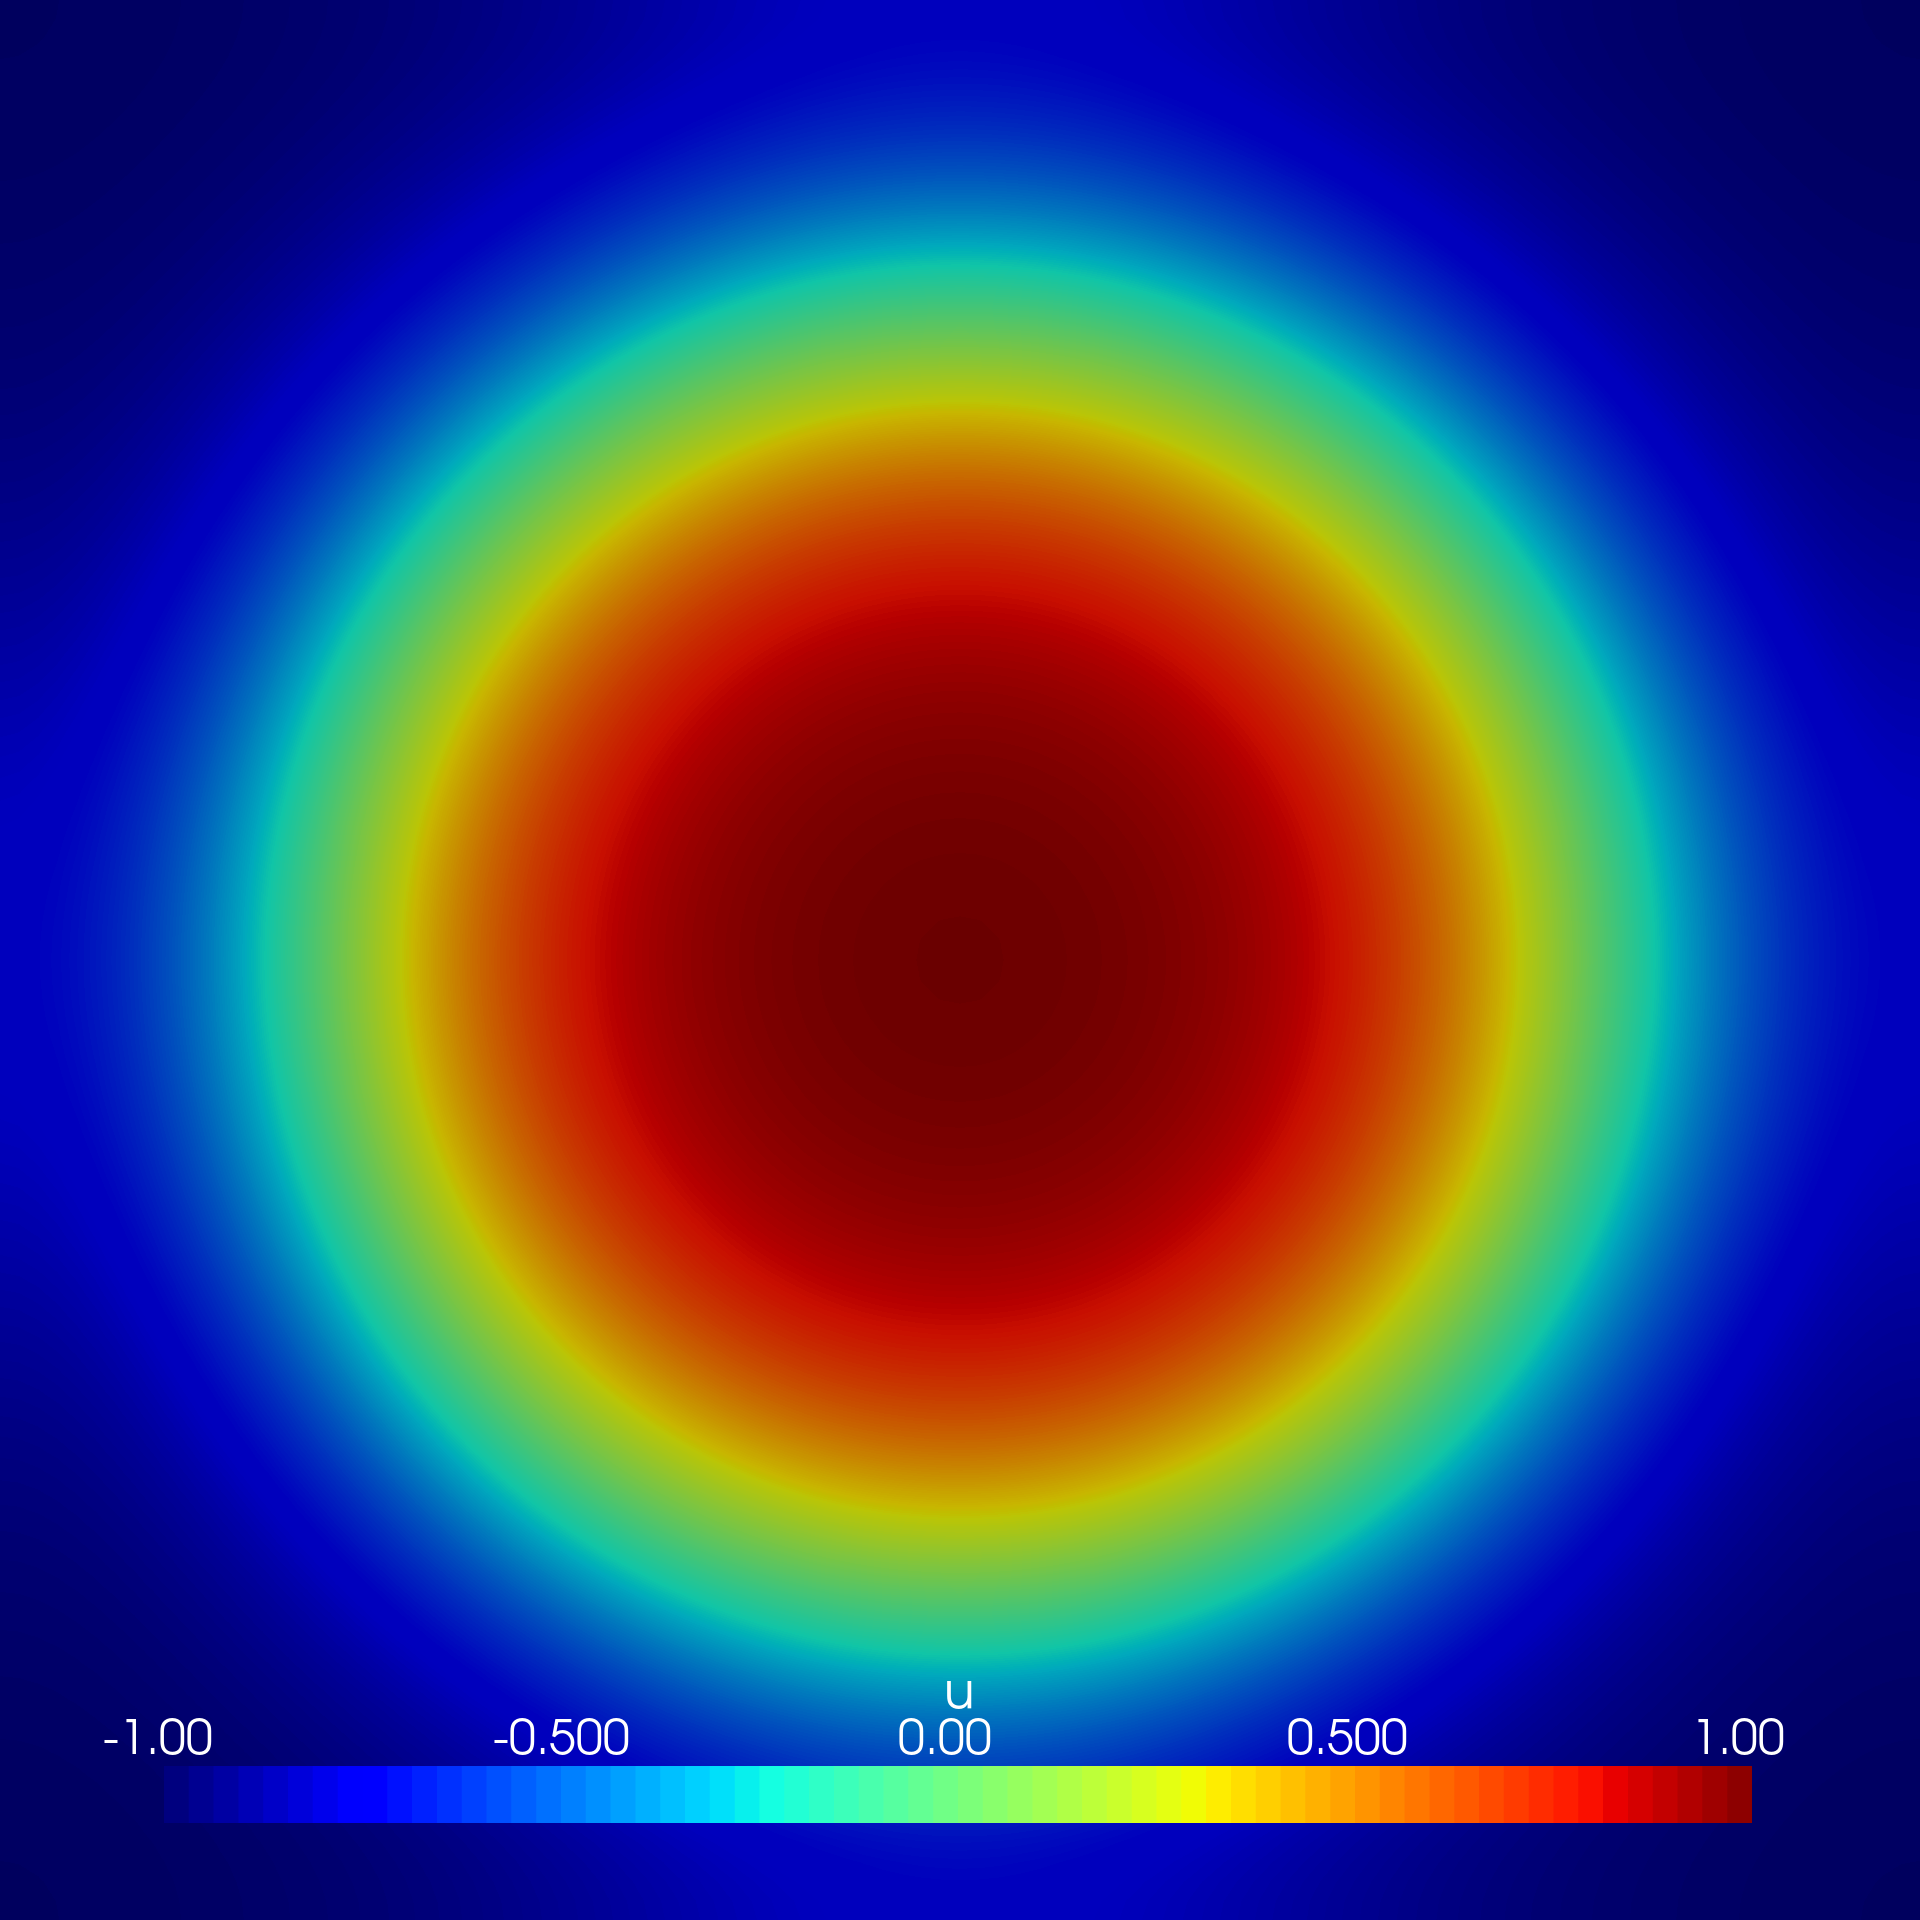
\includegraphics[width=\linewidth]{numerical_simulation/bump/eps_0.2000015.vtu}
		\caption{$ \varepsilon = 0.2, t = 15 dt $}
	\end{subfigure}
	\hfill
	\begin{subfigure}[b]{0.3\linewidth}
		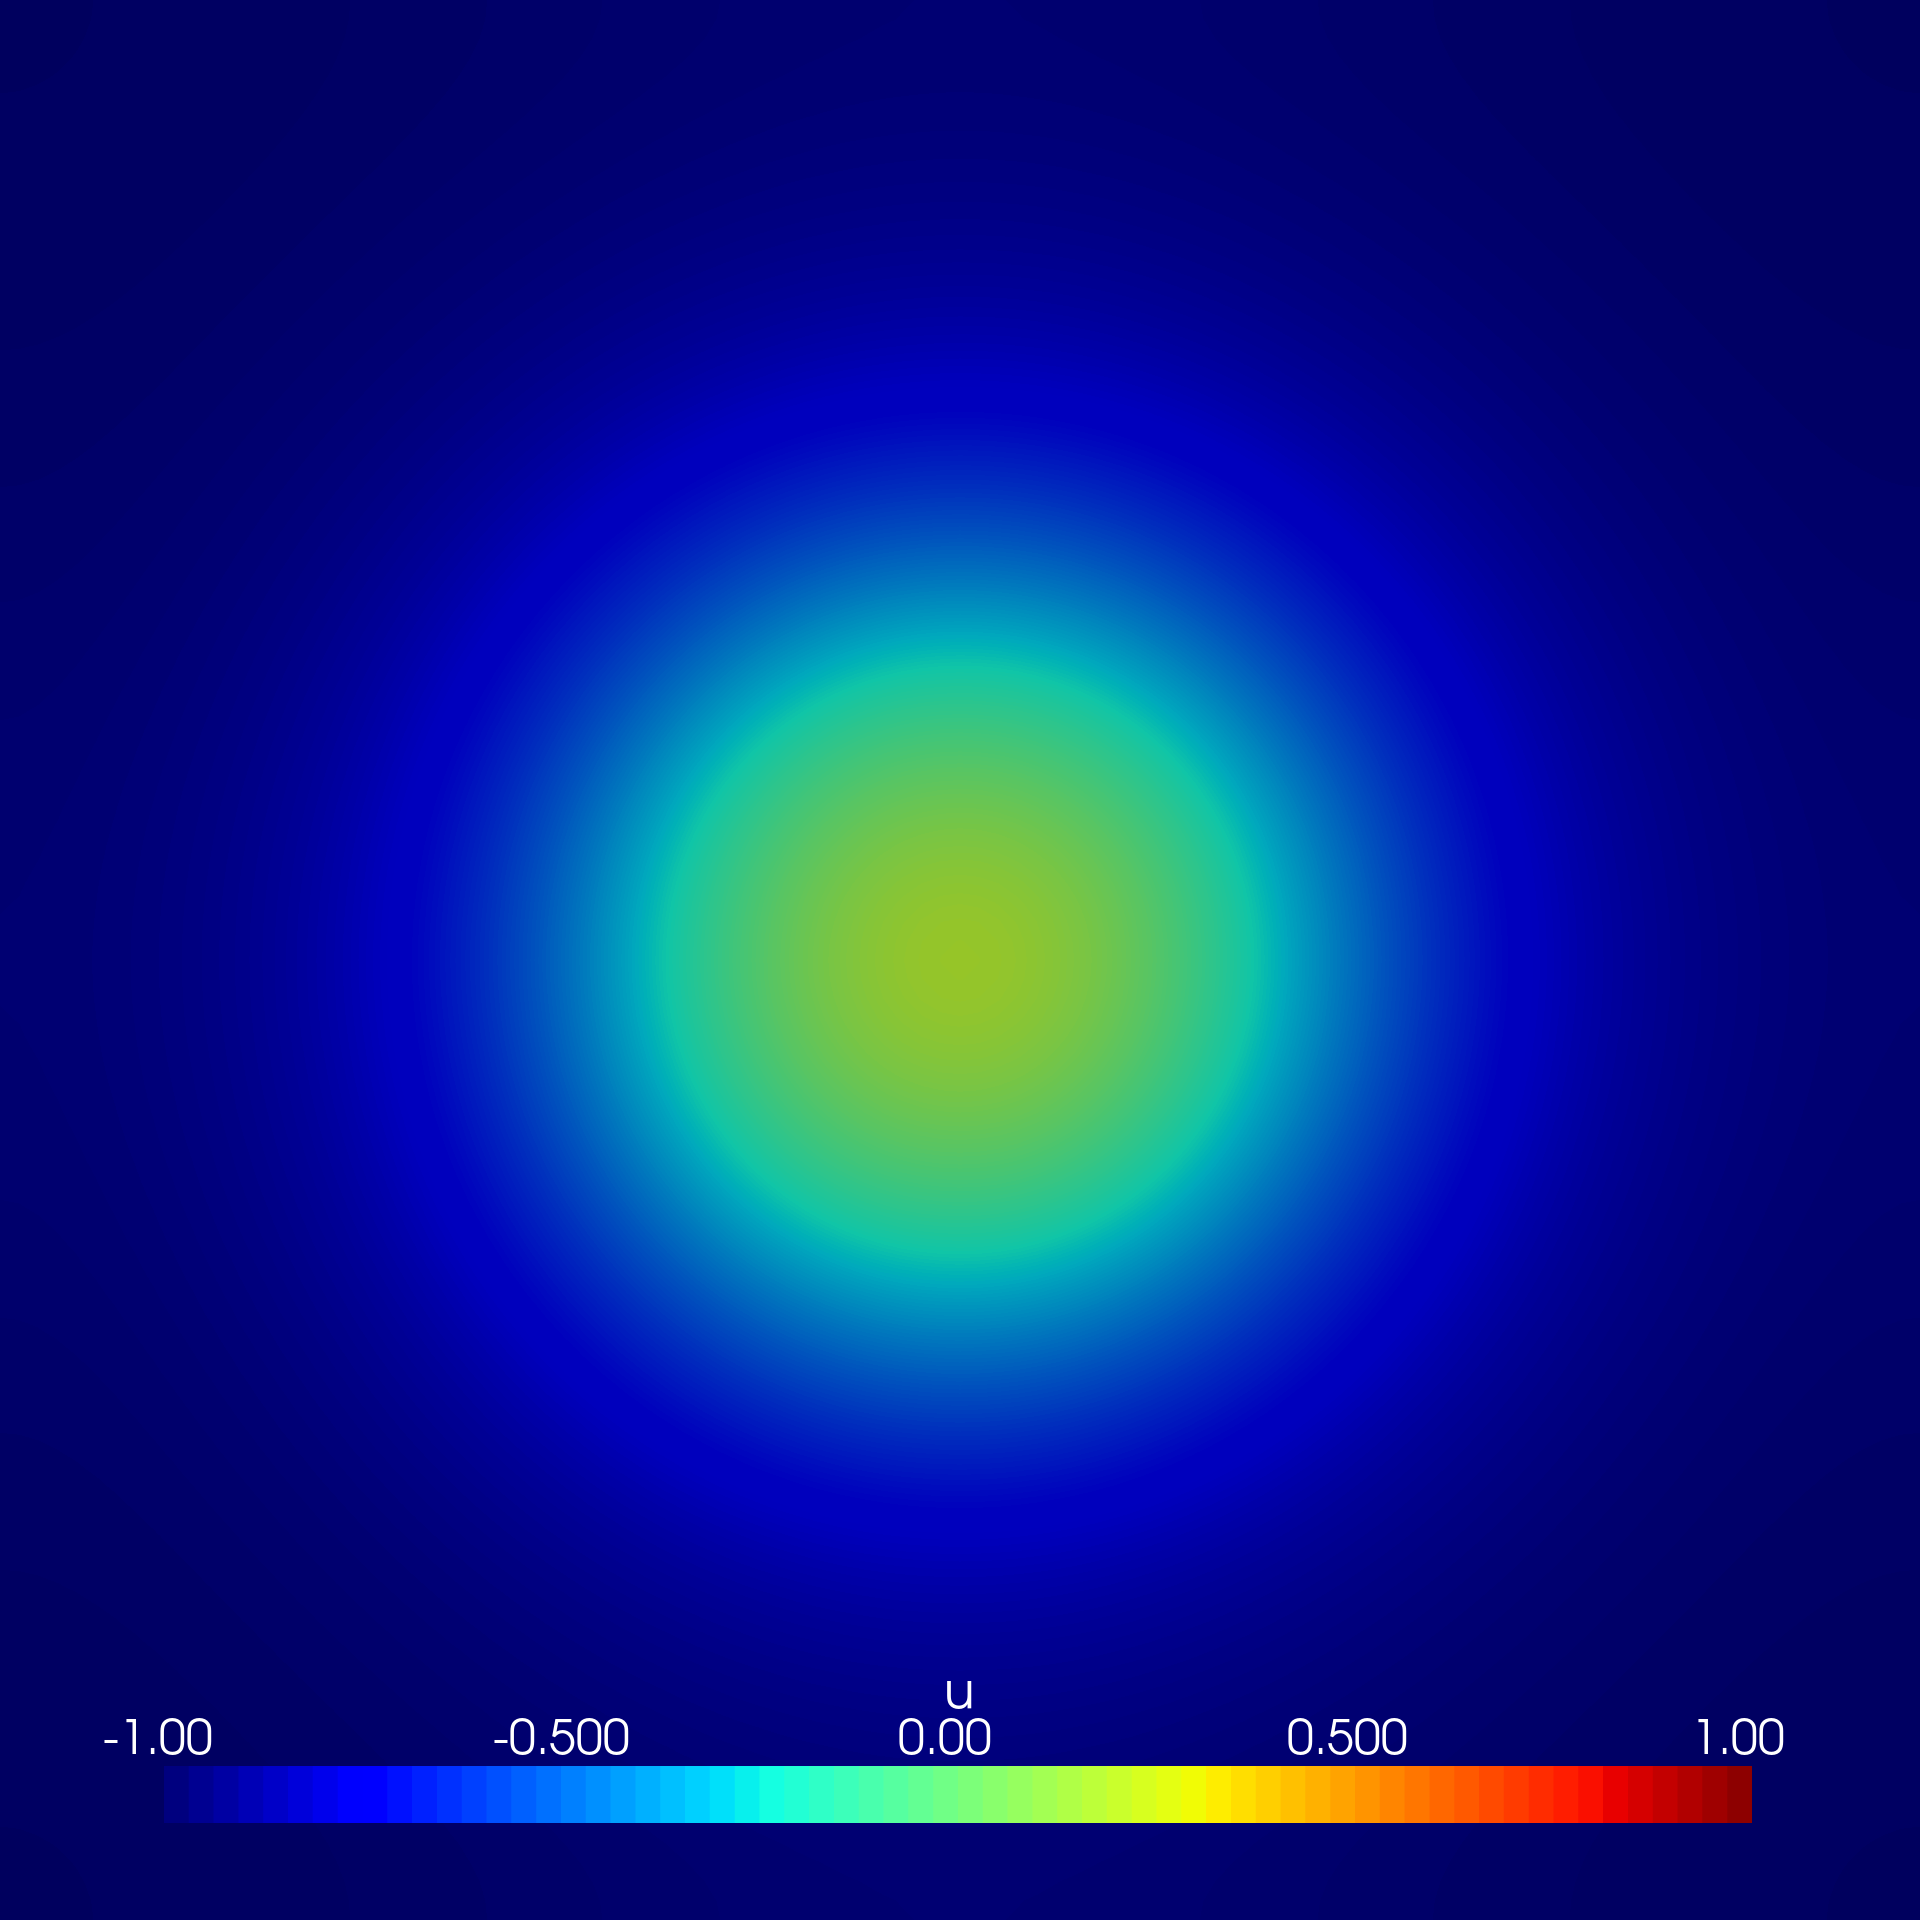
\includegraphics[width=\linewidth]{numerical_simulation/bump/eps_0.2000101.vtu}
		\caption{$ \varepsilon = 0.2, t =  100 dt $}
	\end{subfigure}
	
	\begin{subfigure}[b]{0.3\linewidth}
		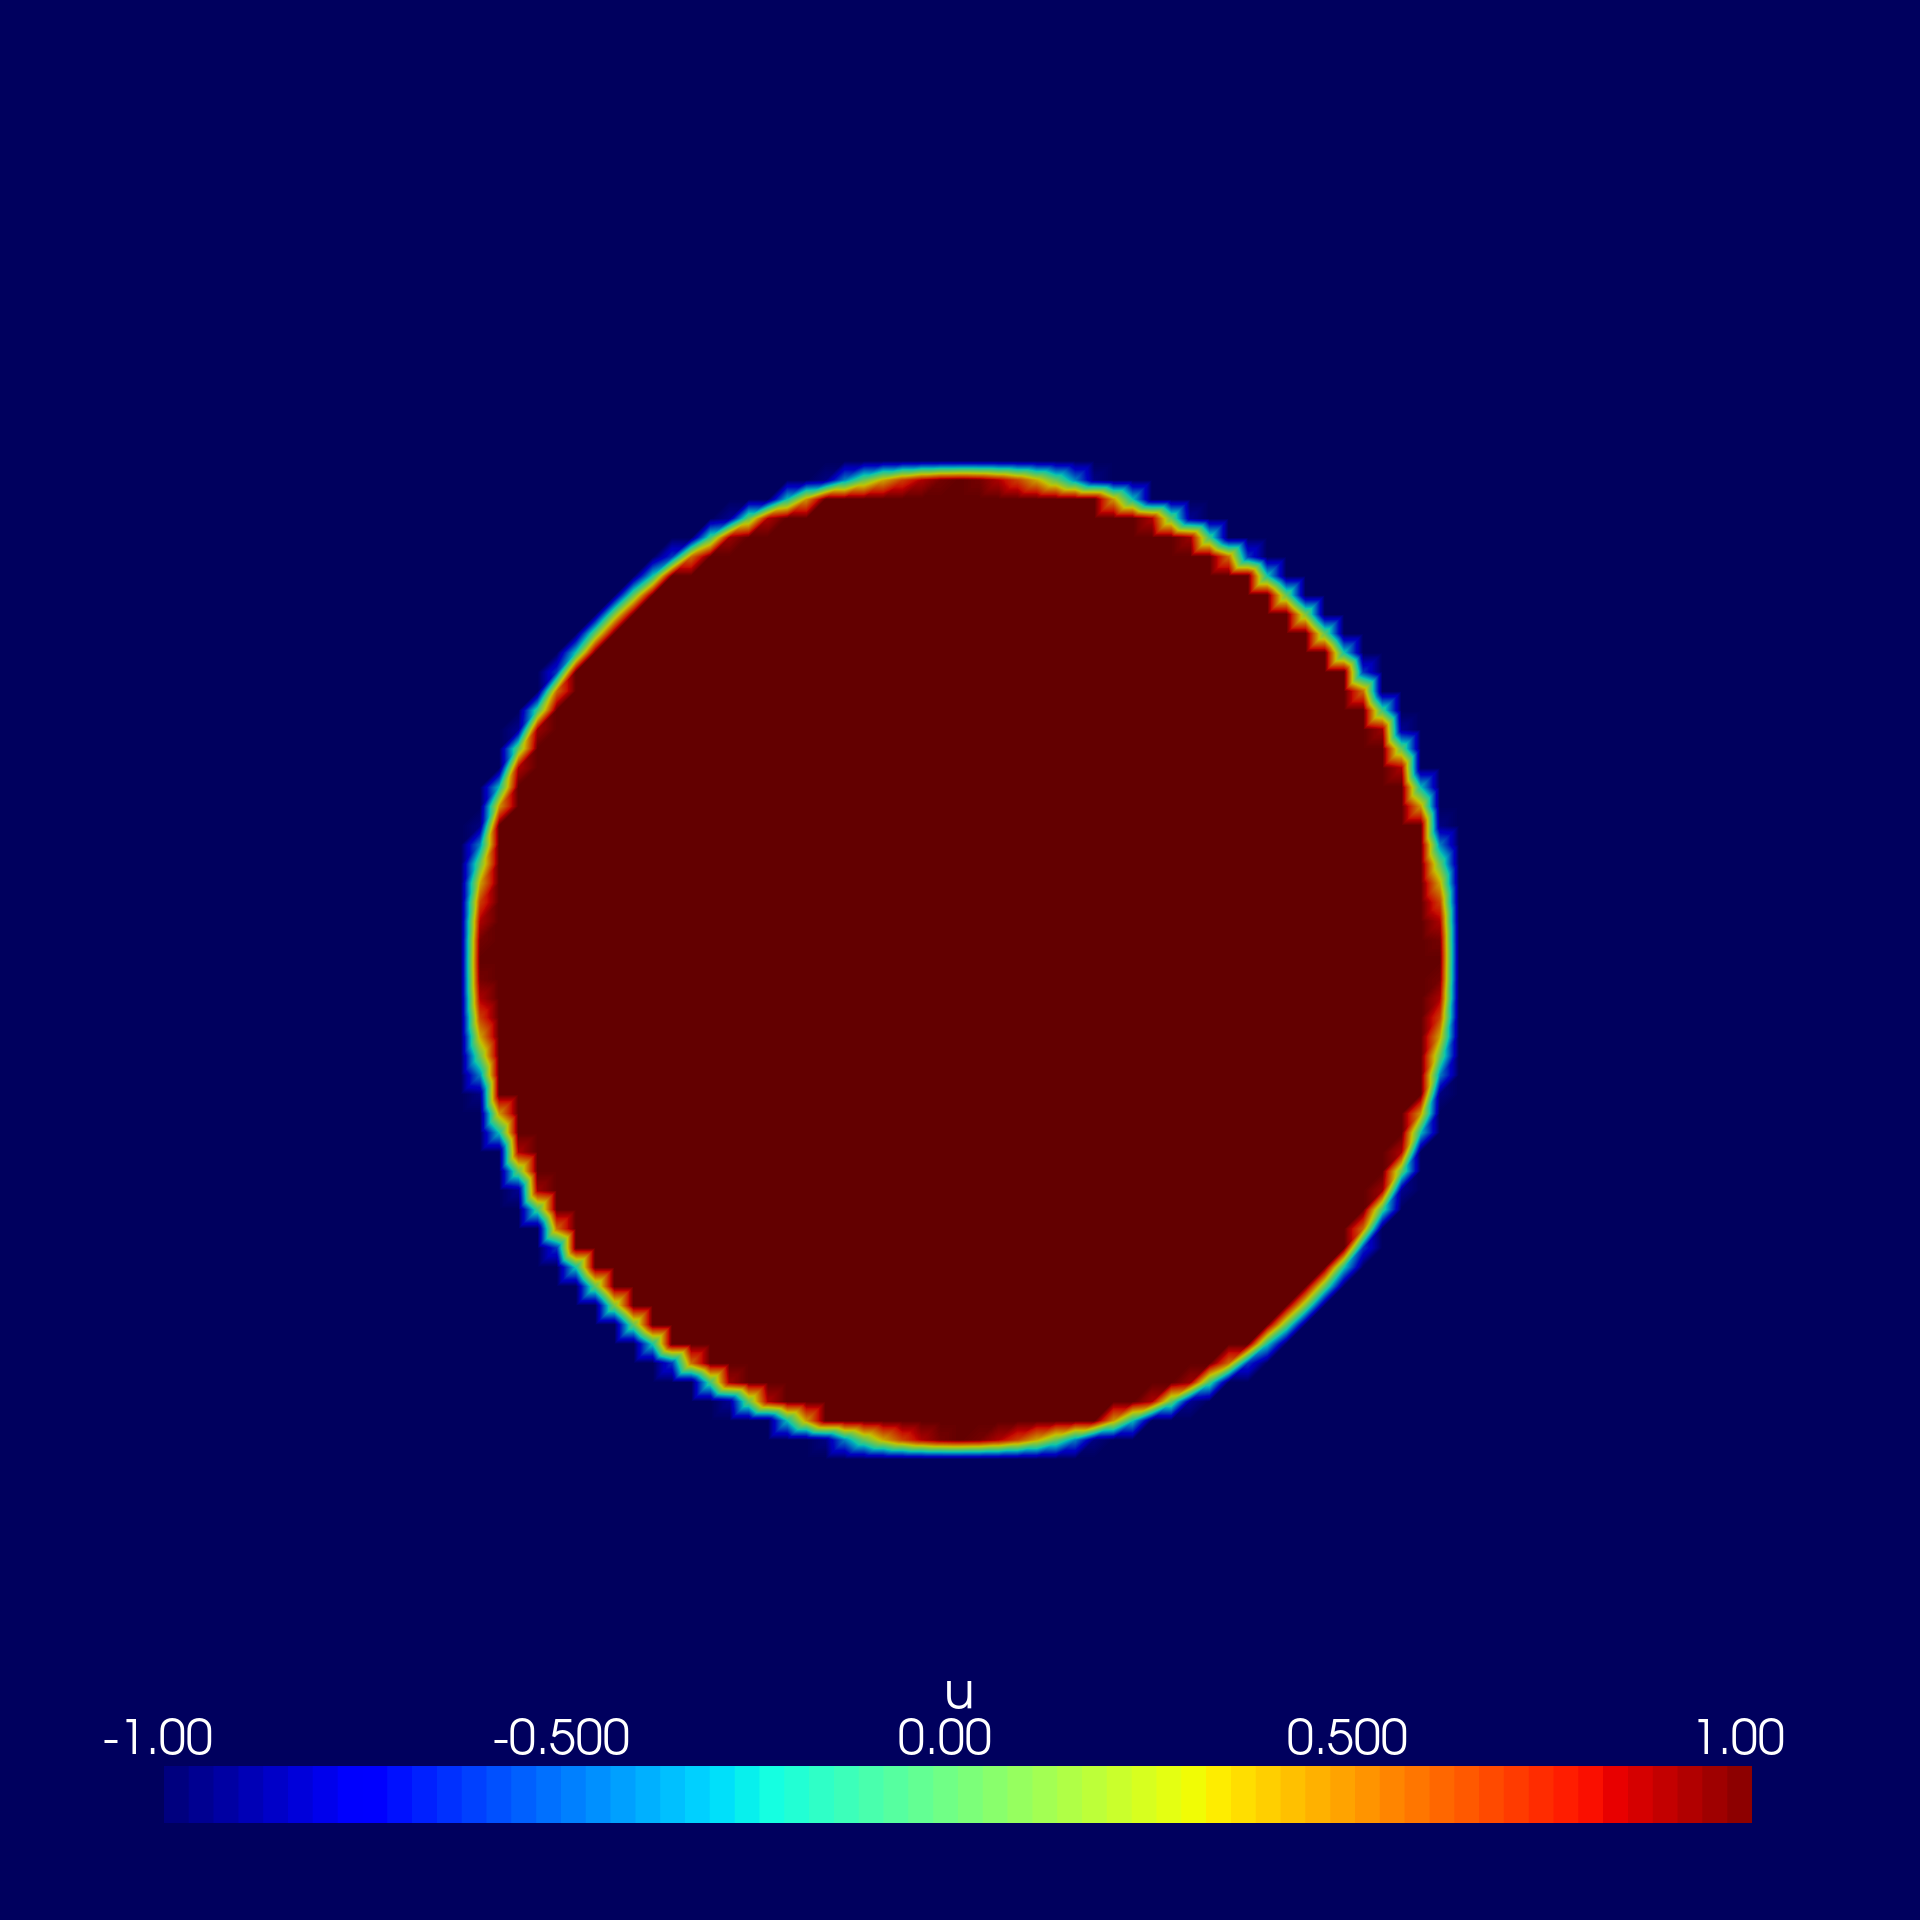
\includegraphics[width=\linewidth]{numerical_simulation/bump/eps_0.01000000.vtu}
		\caption{$ \varepsilon = 0.01, t = 0 $}
	\end{subfigure}
	\hfill
	\begin{subfigure}[b]{0.3\linewidth}
		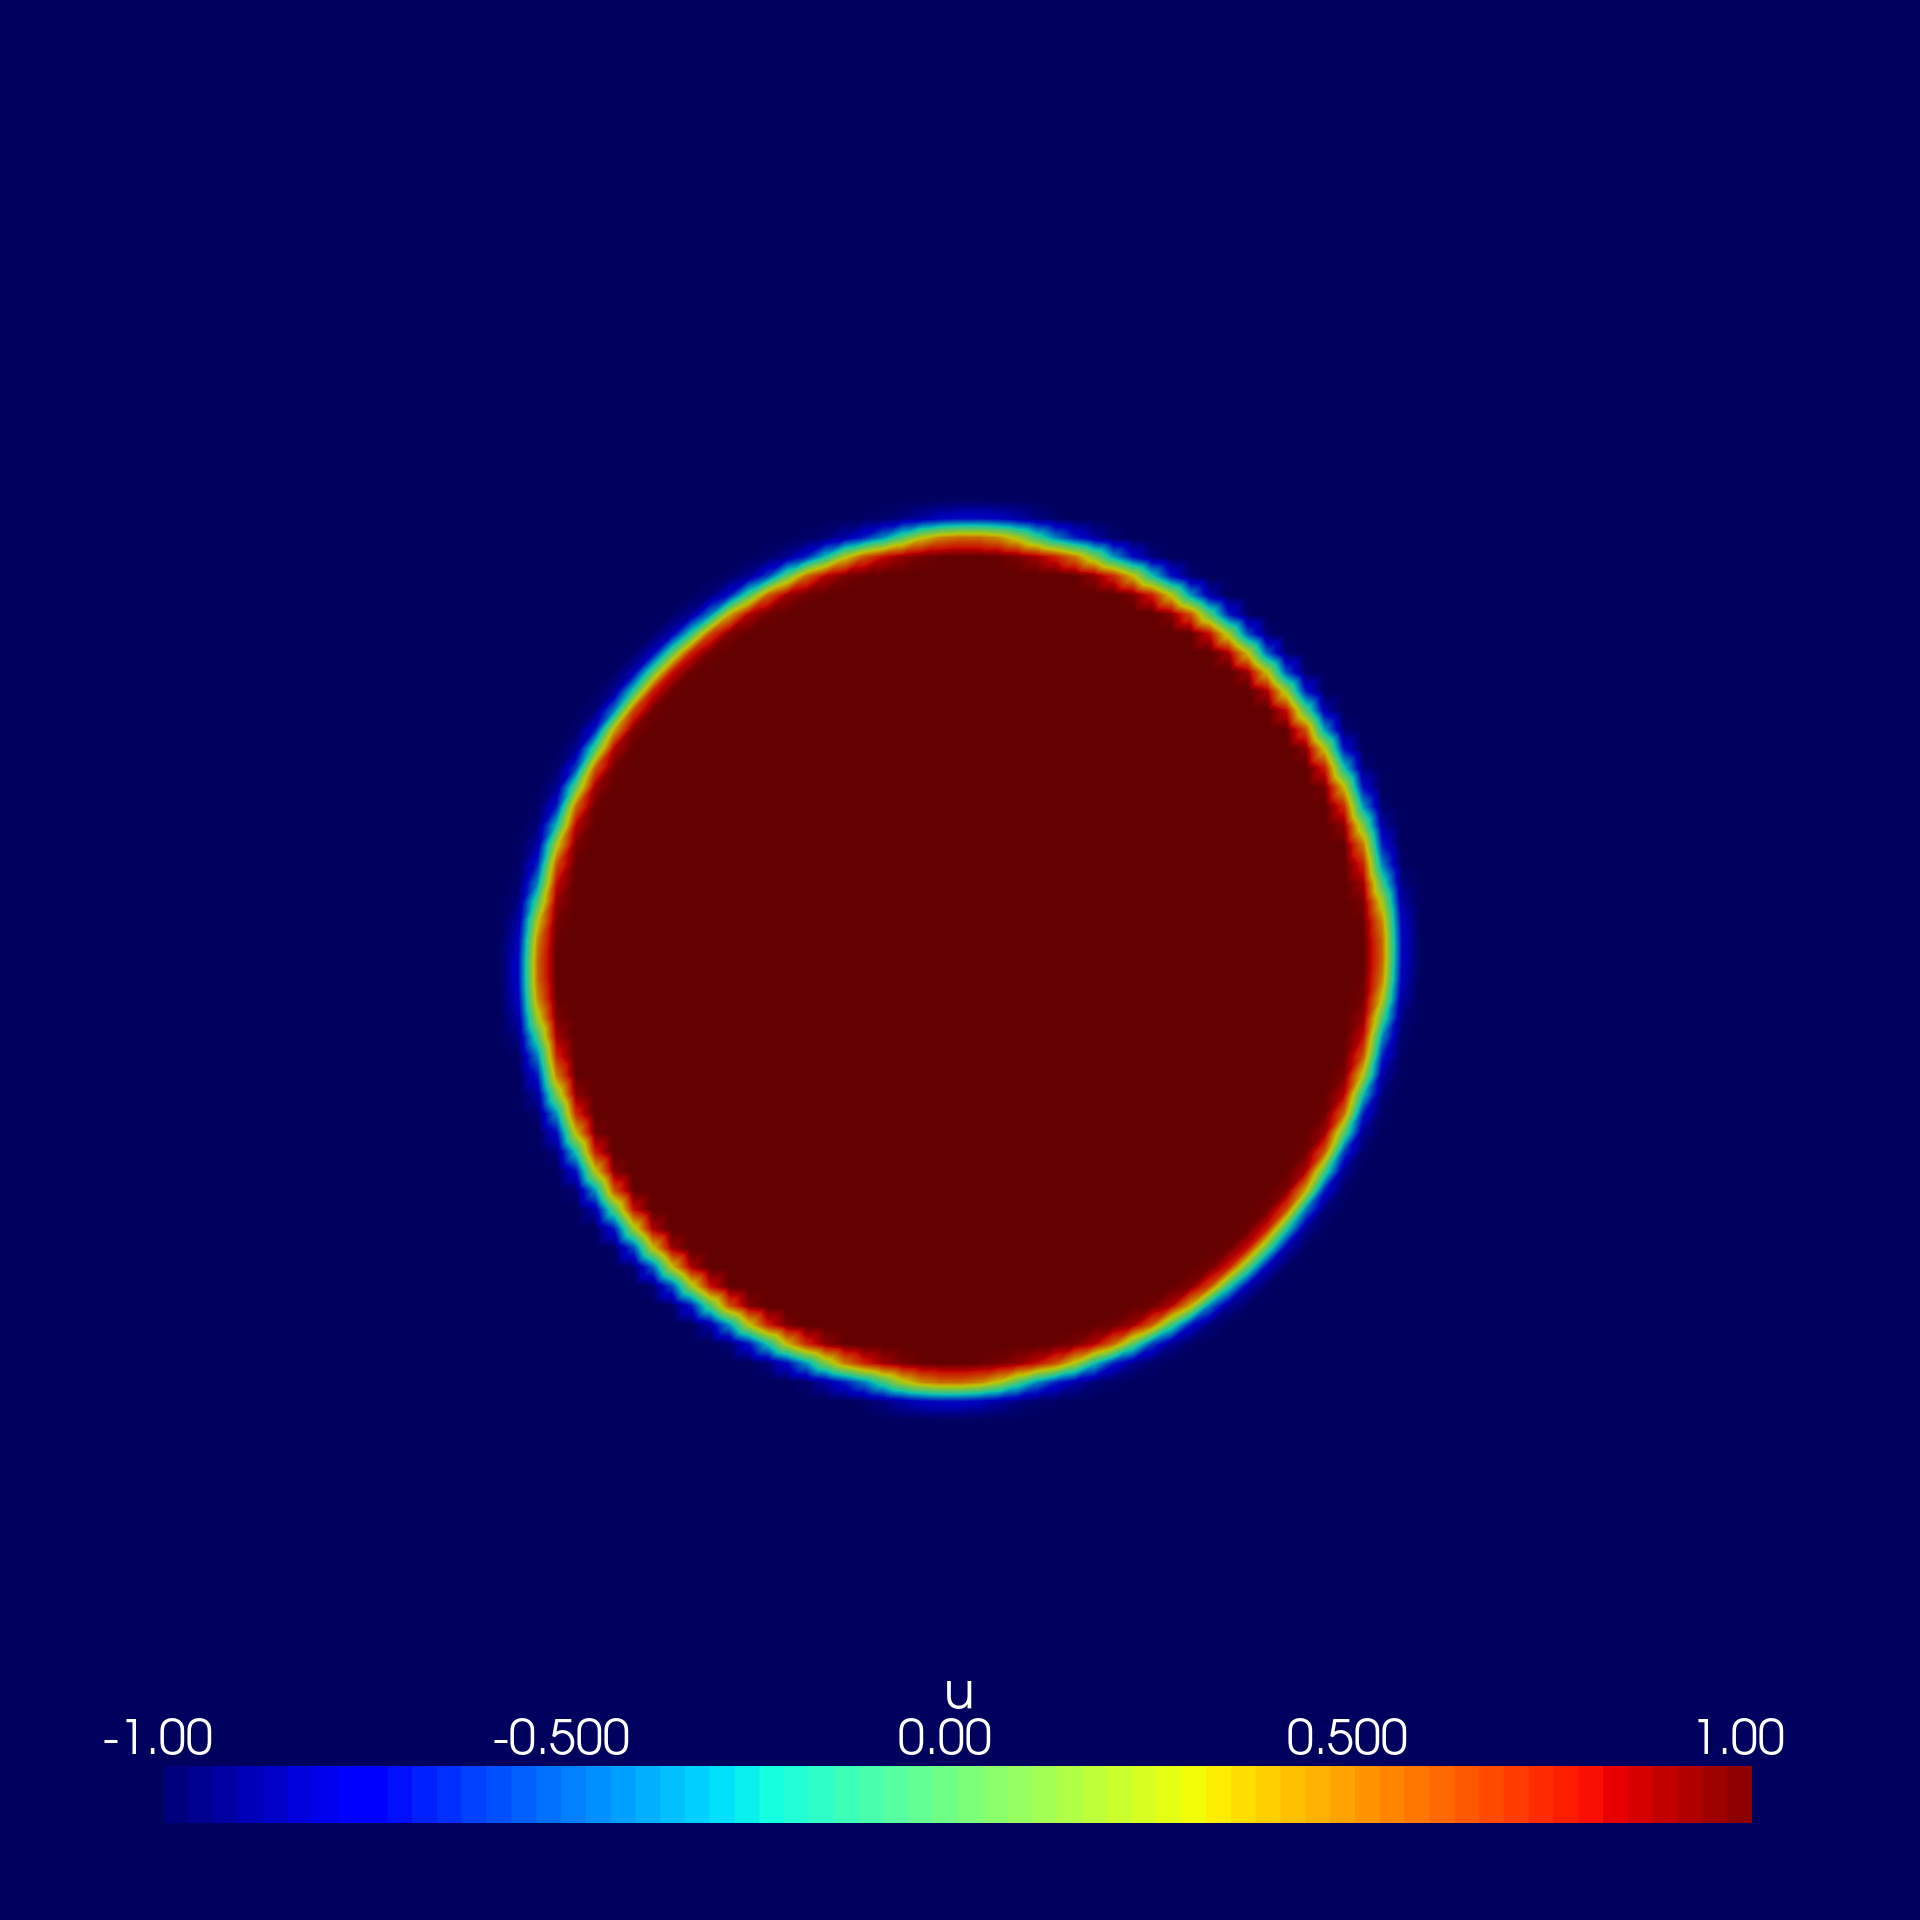
\includegraphics[width=\linewidth]{numerical_simulation/bump/eps_0.01000015.vtu}
		\caption{$ \varepsilon = 0.01, t =15 dt $}
	\end{subfigure}
	\hfill
	\begin{subfigure}[b]{0.3\linewidth}
		\includegraphics[width=\linewidth]{numerical_simulation/bump/eps_0.01000101.vtu}
		\caption{$ \varepsilon = 0.01, t =  100 dt $}
	\end{subfigure}
	
	\caption{Behaviour of the solution $u_{ \varepsilon } $ with an 
	approximated bump function as initial data. For small $ \varepsilon $, the 
	approximate interfaces are rather sharp. For both $ \varepsilon $, we see 
	that 
	the ball shrinks to a single point and vanishes, as one would expect for 
	mean curvature flow}
	\label{numerical_simulation_bump}
\end{figure}

\begin{figure}[h]
	\centering
	
	\begin{subfigure}[b]{0.3\linewidth}
		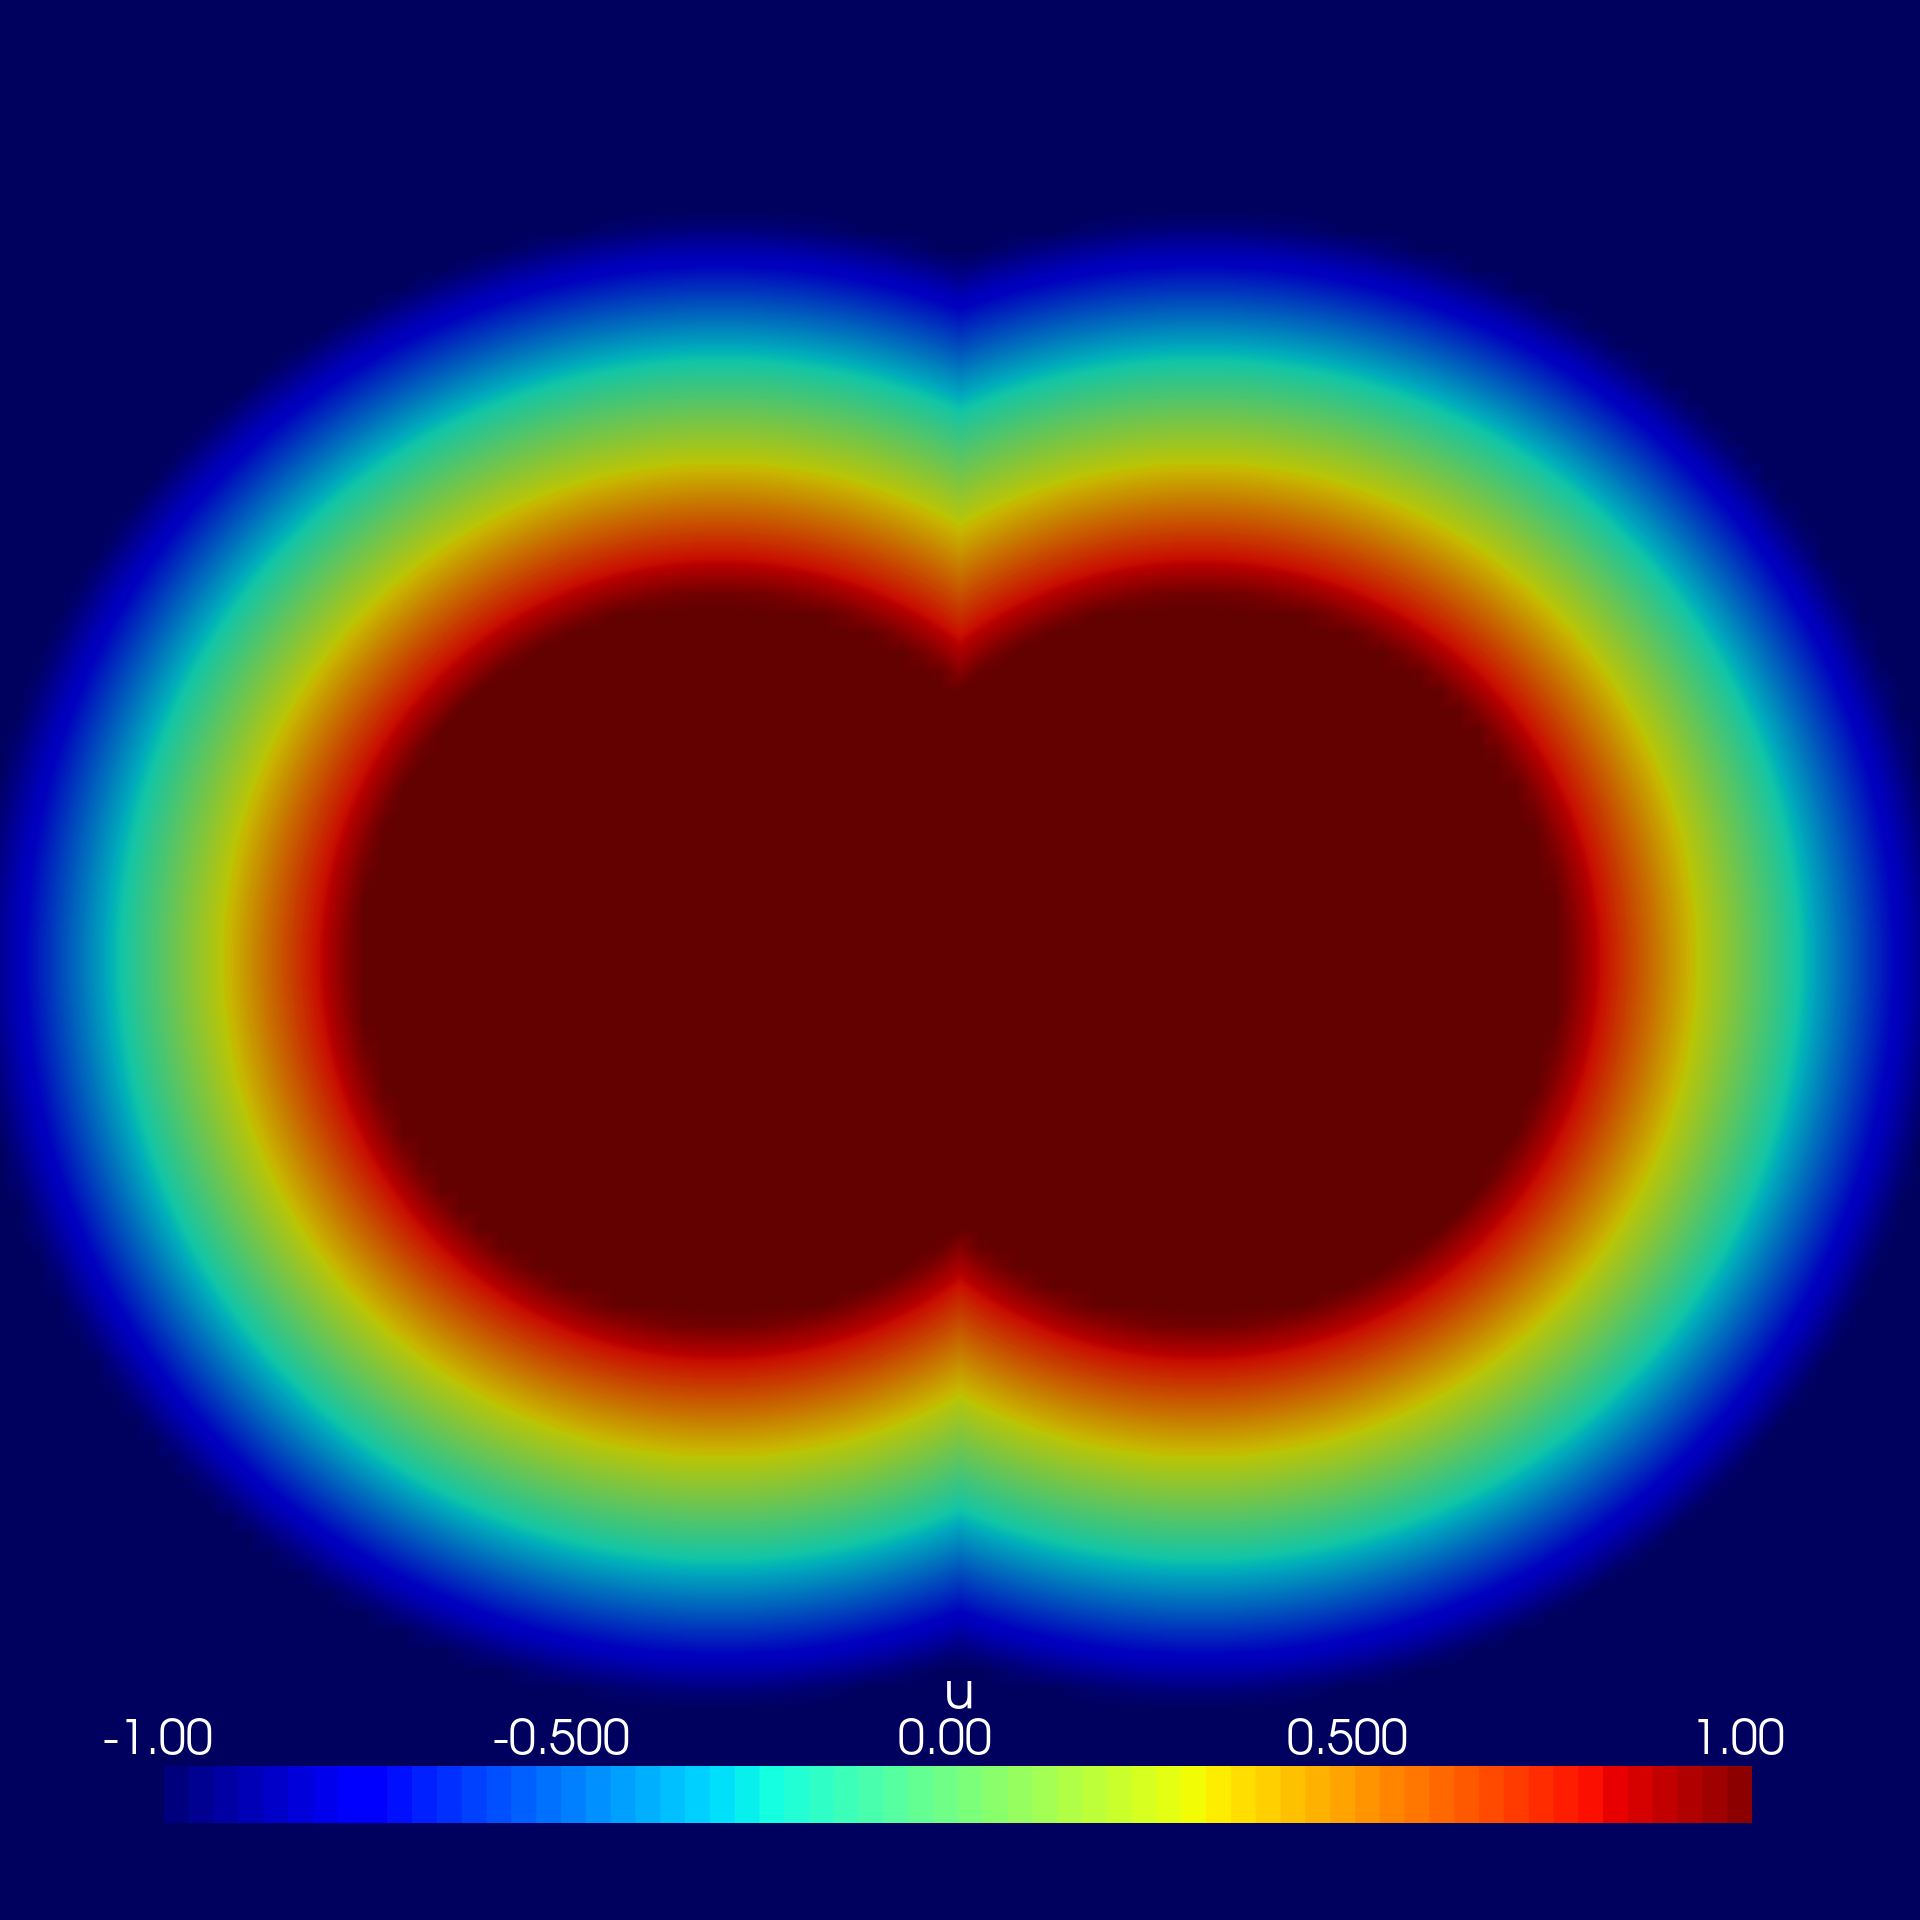
\includegraphics[width=\linewidth]{numerical_simulation/dumbel/eps_0.2000000.vtu}
		\caption{$ \varepsilon = 0.2, t = 0 $}
	\end{subfigure}
	\hfill
	\begin{subfigure}[b]{0.3\linewidth}
		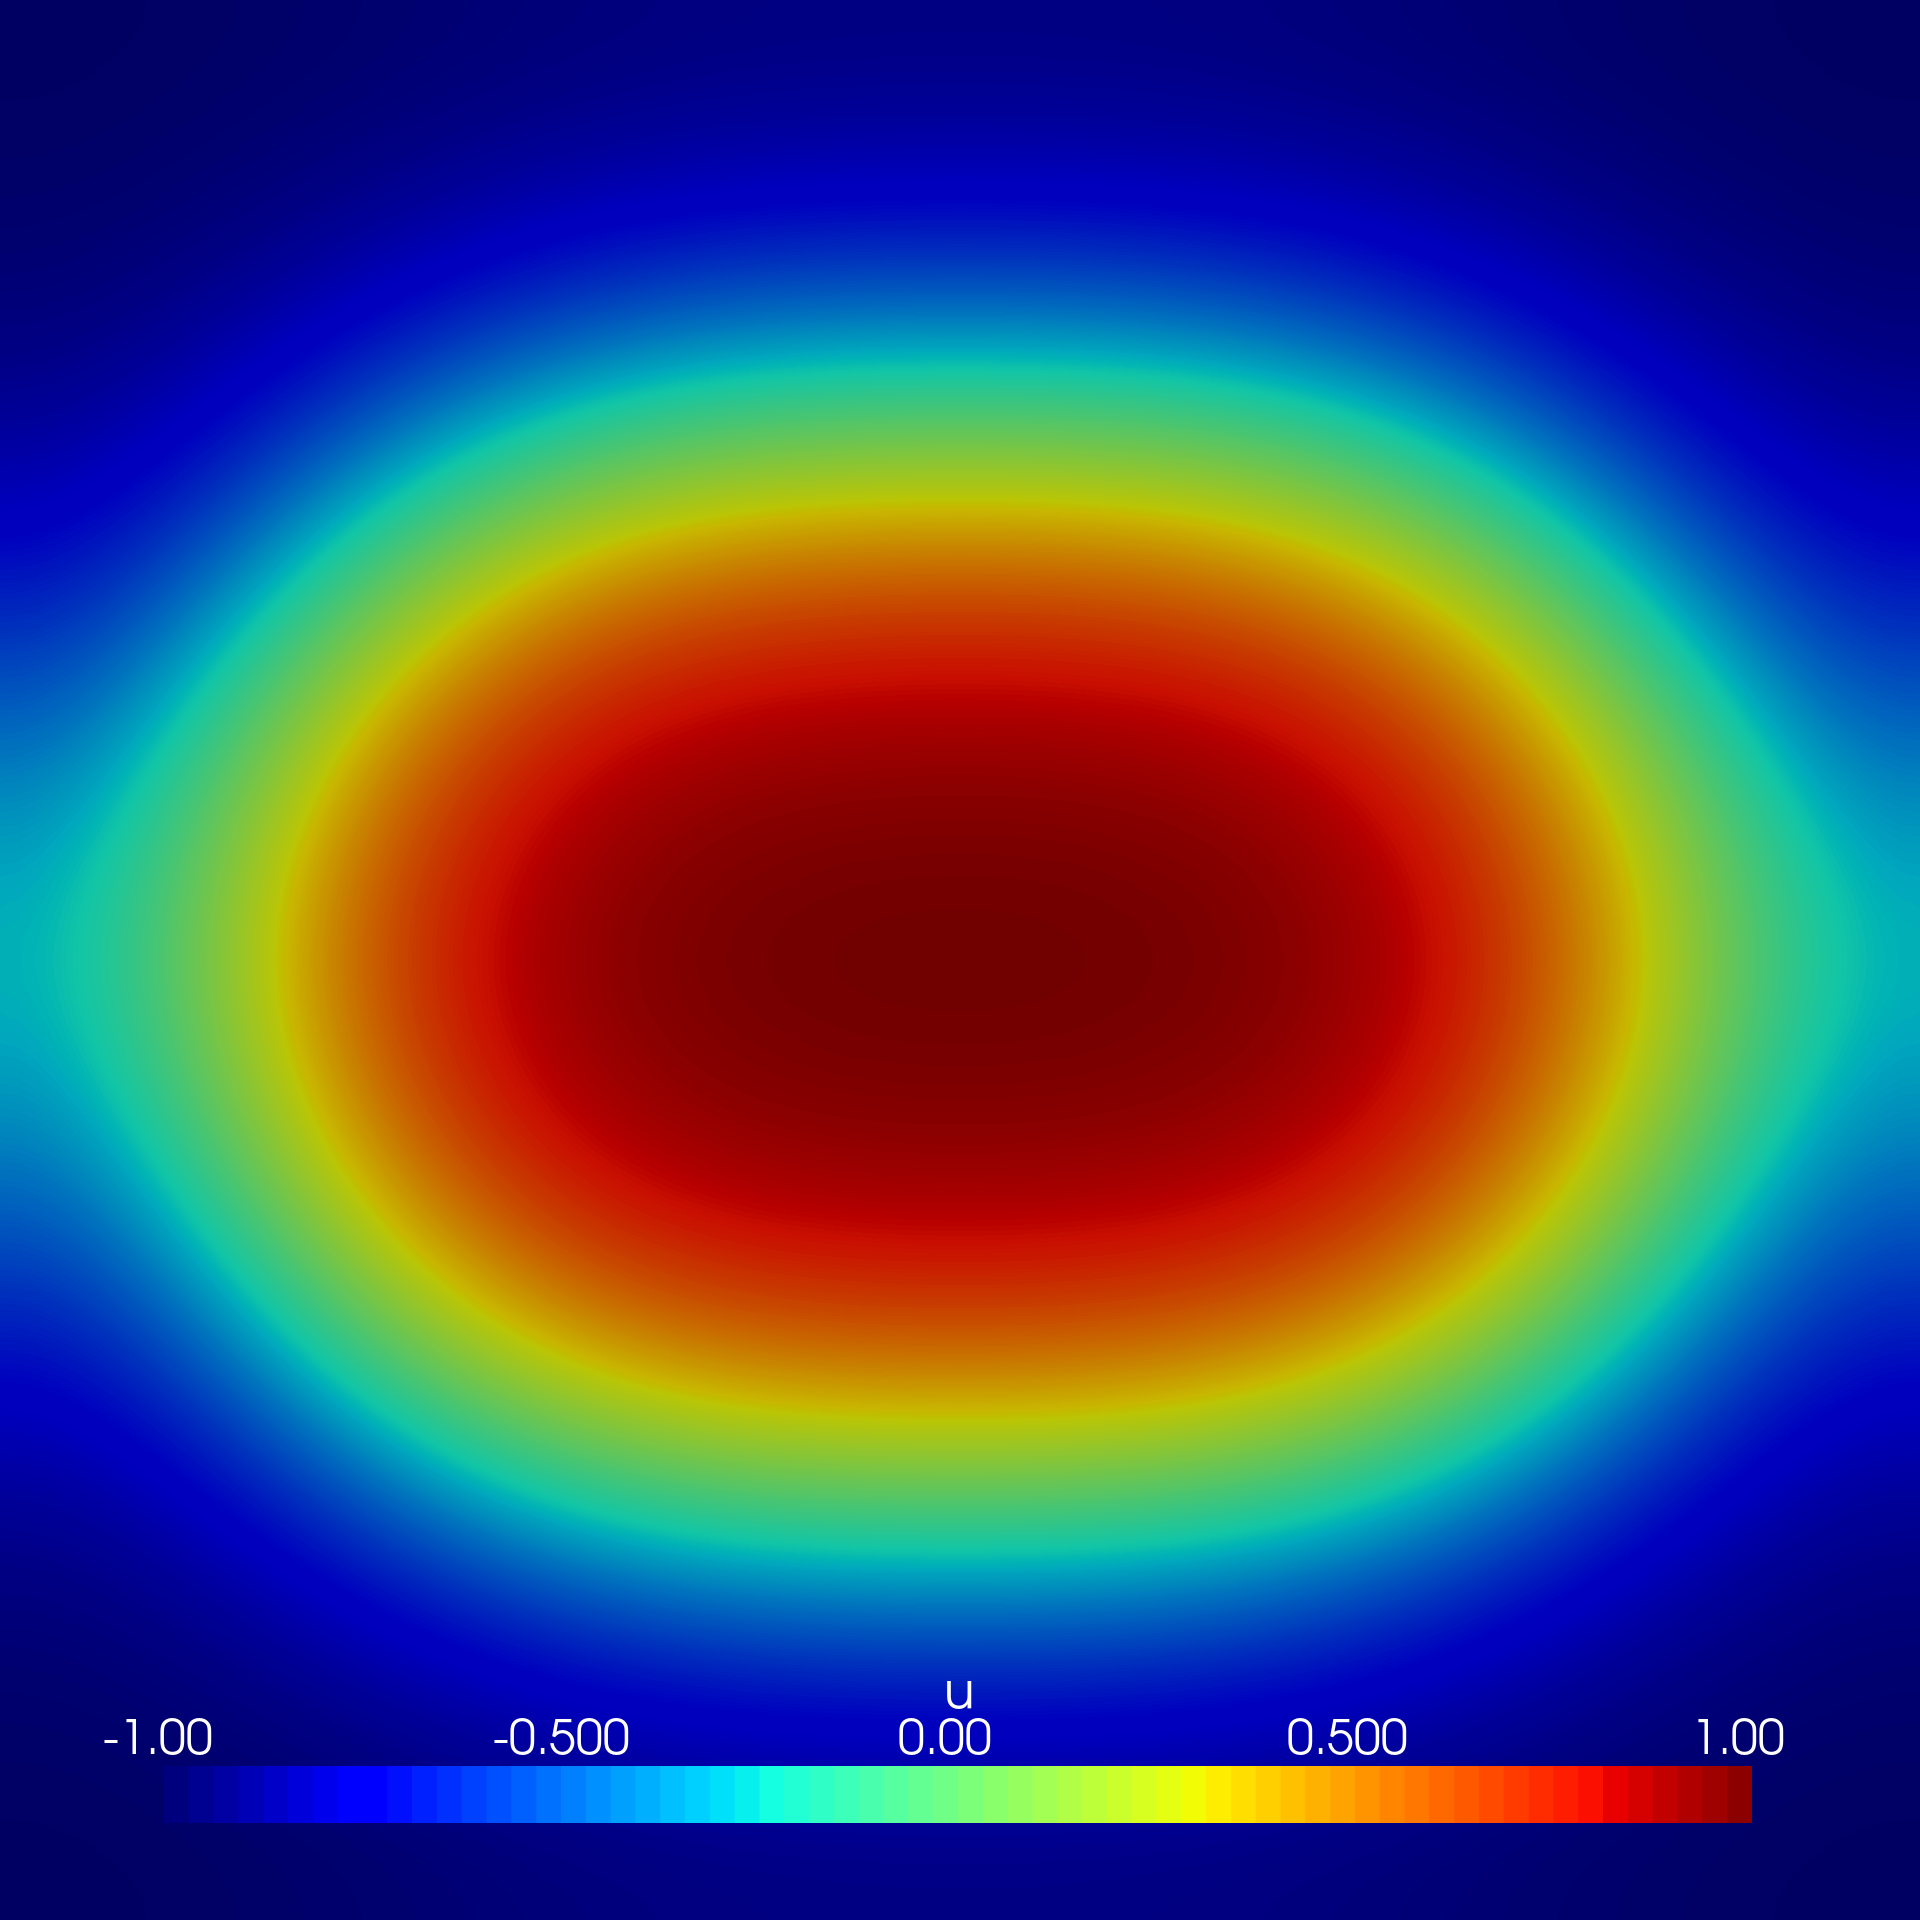
\includegraphics[width=\linewidth]{numerical_simulation/dumbel/eps_0.2000015.vtu}
		\caption{$ \varepsilon = 0.2, t = 15dt $}
	\end{subfigure}
	\hfill
	\begin{subfigure}[b]{0.3\linewidth}
		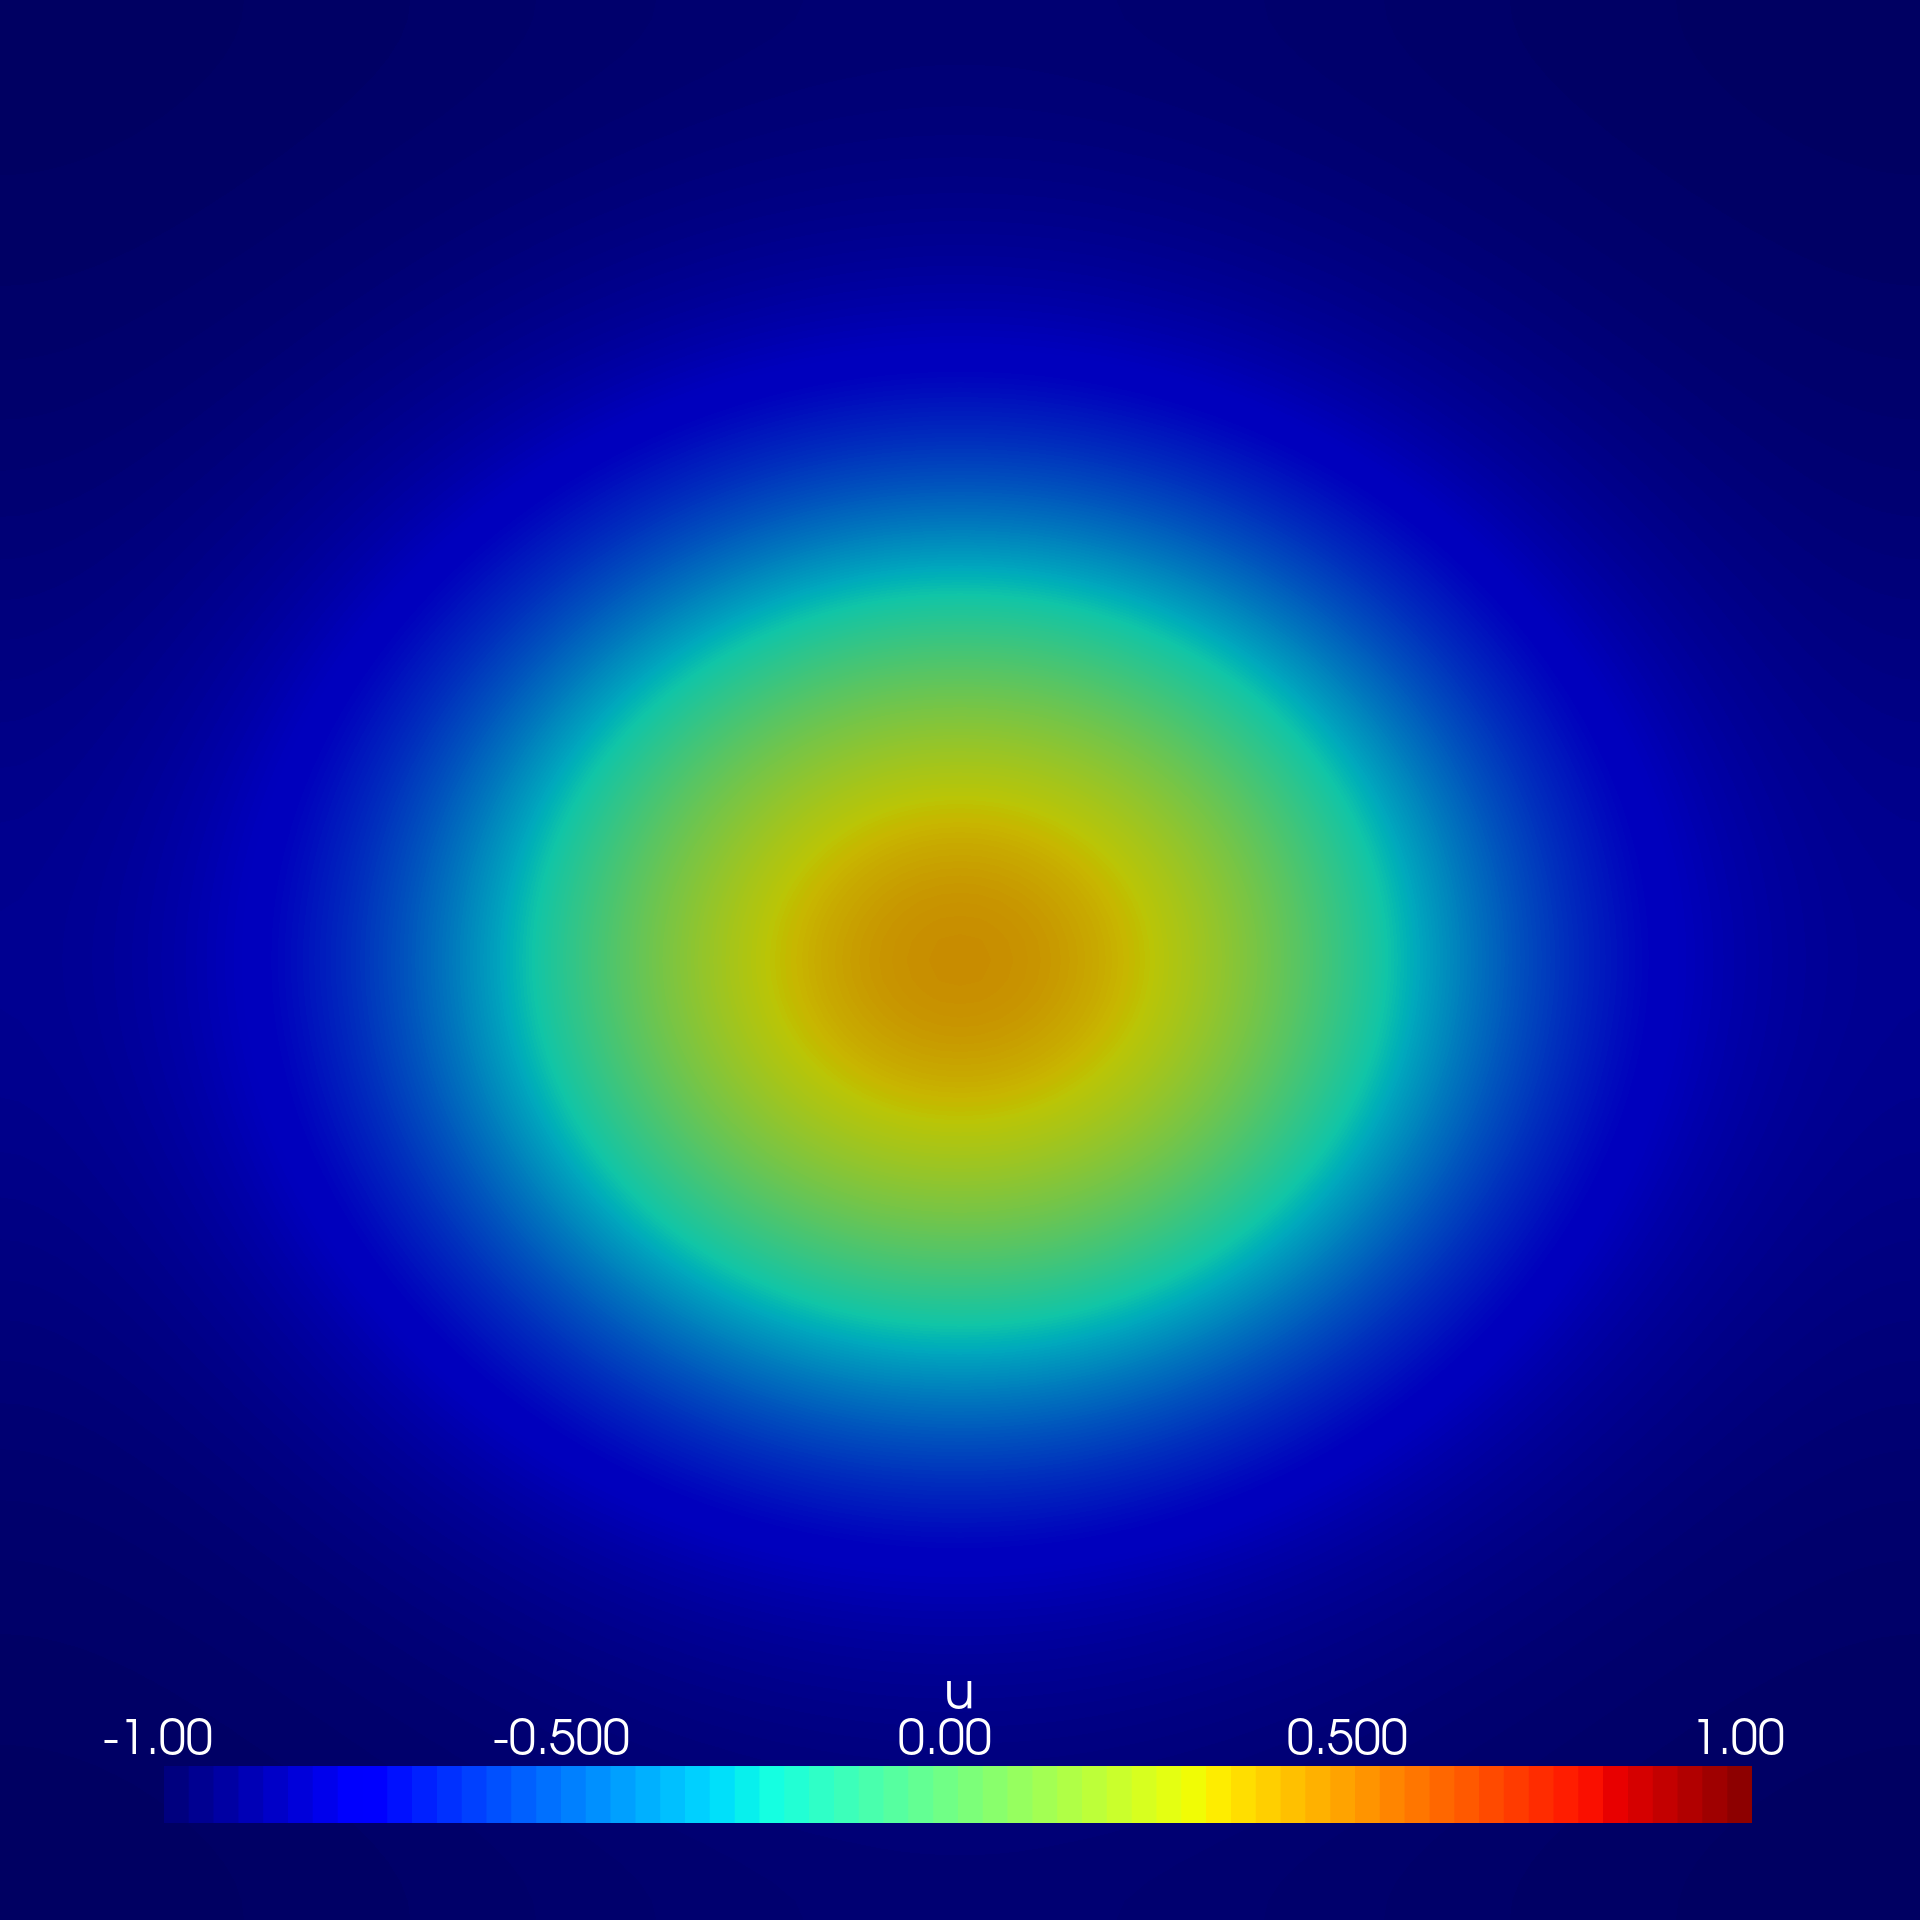
\includegraphics[width=\linewidth]{numerical_simulation/dumbel/eps_0.2000101.vtu}
		\caption{$ \varepsilon = 0.2, t =  100dt $}
	\end{subfigure}
	
	\begin{subfigure}[b]{0.3\linewidth}
		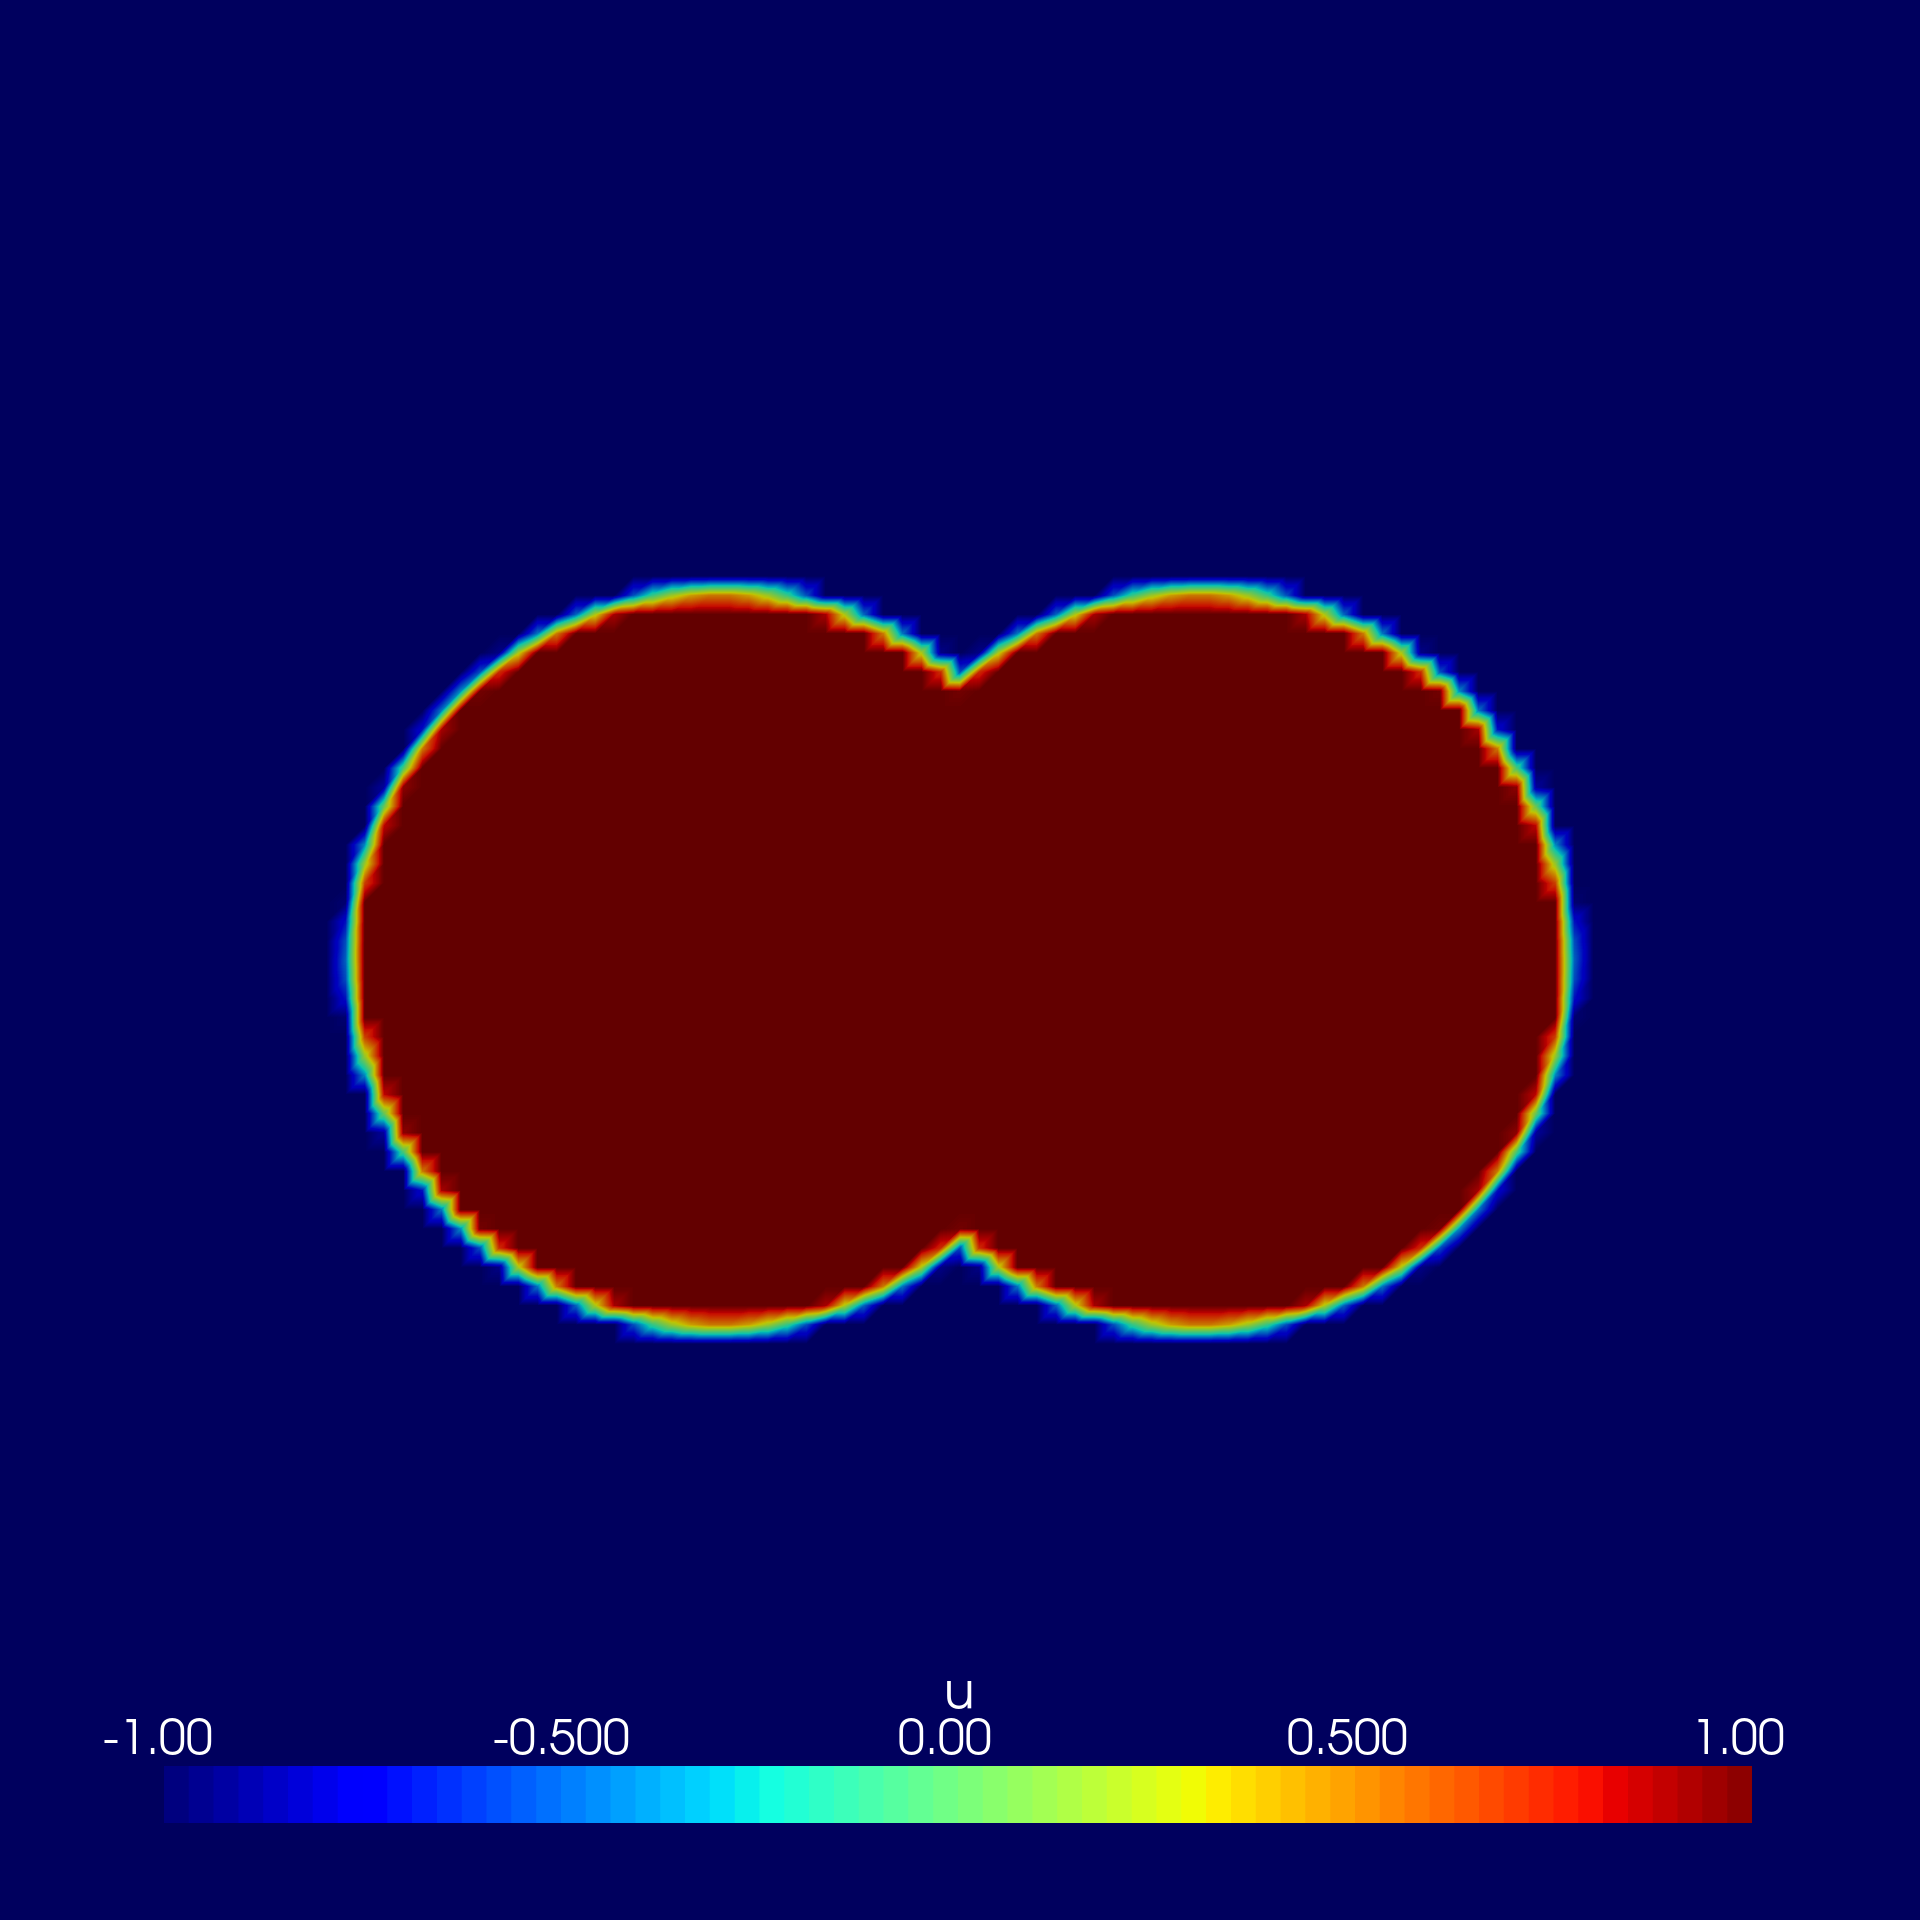
\includegraphics[width=\linewidth]{numerical_simulation/dumbel/eps_0.01000000.vtu}
		\caption{$ \varepsilon = 0.01, t = 0 $}
	\end{subfigure}
	\hfill
	\begin{subfigure}[b]{0.3\linewidth}
		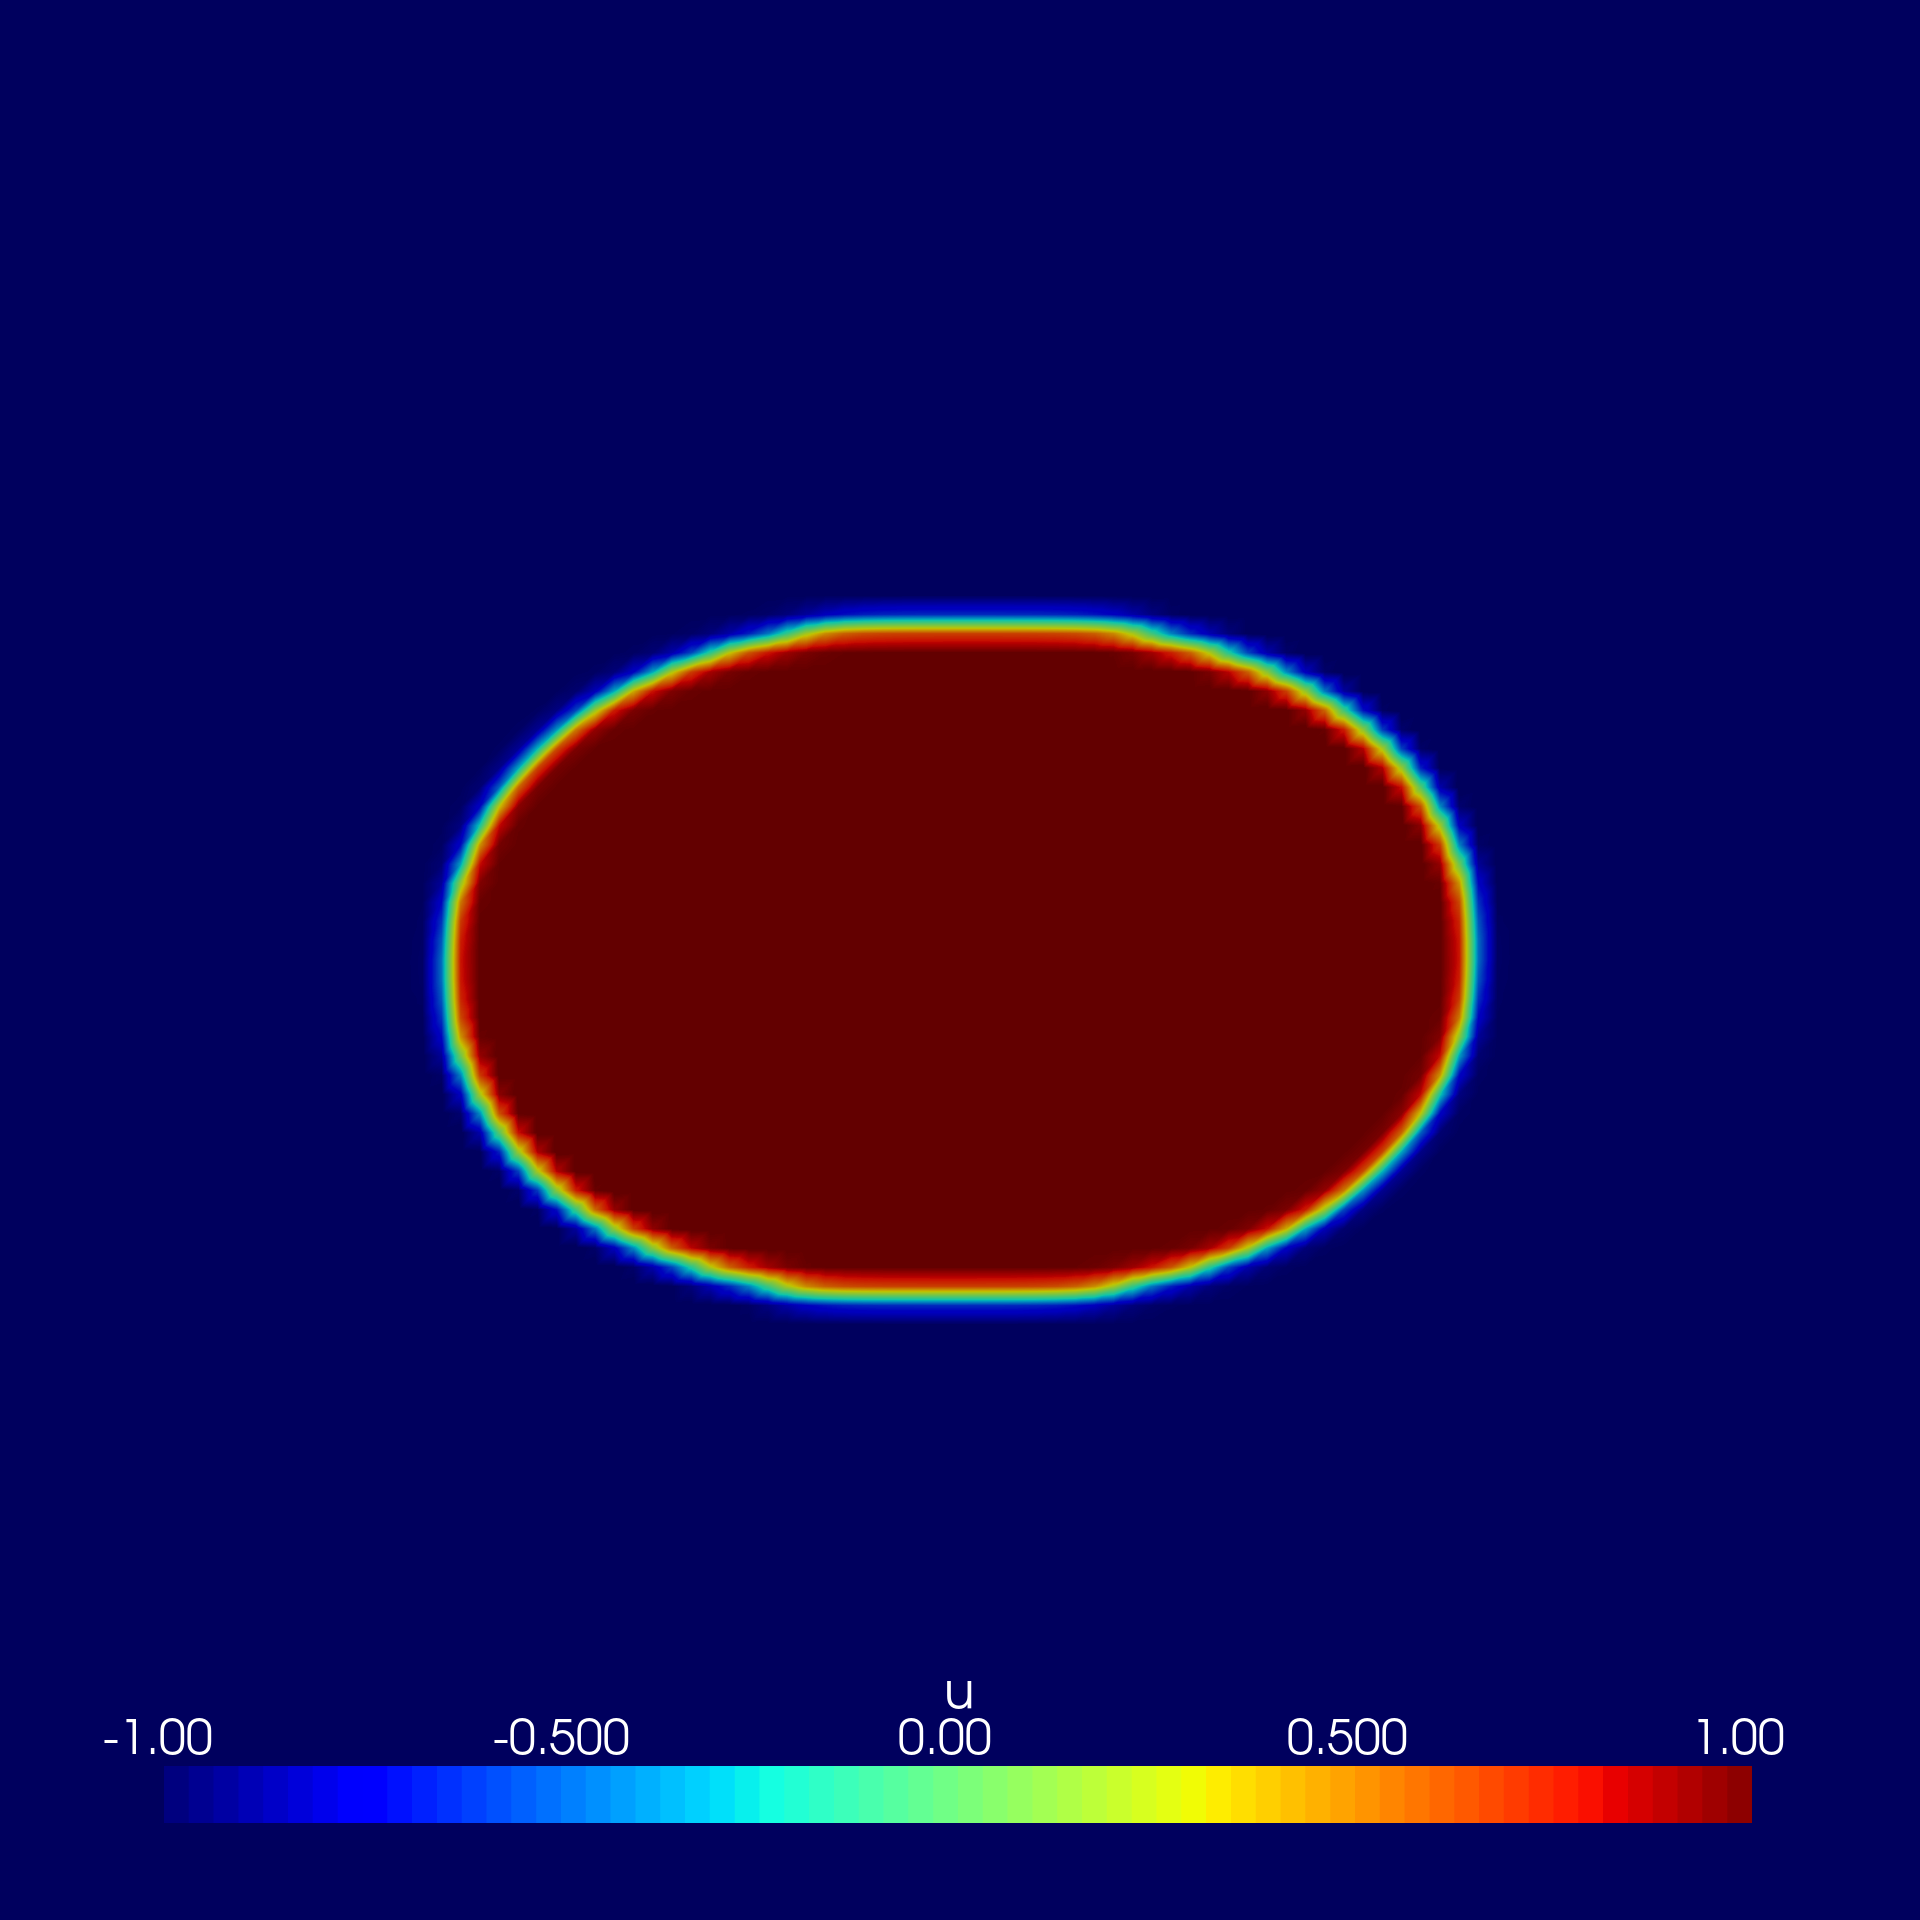
\includegraphics[width=\linewidth]{numerical_simulation/dumbel/eps_0.01000015.vtu}
		\caption{$ \varepsilon = 0.01, t = 15dt $}
	\end{subfigure}
	\hfill
	\begin{subfigure}[b]{0.3\linewidth}
		\includegraphics[width=\linewidth]{numerical_simulation/dumbel/eps_0.01000101.vtu}
		\caption{$ \varepsilon = 0.01, t =  100dt $}
	\end{subfigure}
	
	\caption{Behaviour of the solution $u_{ \varepsilon } $ with an 
	approximated dumbbell function as initial data. The approximate indicator 
	function first becomes convex, and then shrinks to a single point before 
	vanishing.}
	\label{numerical_simulation_dumbbell}
\end{figure}